\ifx\wholebook\relax \else

\documentclass[b5paper]{ctexart}
\usepackage[nomarginpar
  %, margin=.5in
]{geometry}

\addtolength{\oddsidemargin}{-0.05in}
\addtolength{\evensidemargin}{-0.05in}
\addtolength{\textwidth}{0.1in}

\usepackage[cn]{../prelude}

\setcounter{page}{1}

\begin{document}

\title{分数}

\author{刘新宇
\thanks{{\bfseries 刘新宇} \newline
  Email: liuxinyu99@hotmail.com \newline}
  }

\maketitle
\fi

\markboth{分数}{数的旅程}

\ifx\wholebook\relax
\chapter{分数}
\fi

\epigraph{此曲只应天上有,人间能得几回闻。}{杜甫《赠花卿》}

\index{引力波}
2015年9月14日,美国LIGO\footnote{激光干涉引力波}天文台探测到一个神秘信号GW150914。它来自13亿光年之外的一次惊天动地的奇观:一对双黑洞天体彼此靠近、吸引,旋转着合并到一起(如图\ref{fig:gravitational-wave})。它们巨大引力激起的“涟漪”穿越13亿年时空\footnote{根据爱因斯坦的广义相对论,引力波以光速传播。}到达了地球。物理学家们花了几个月的时间进行数据分析,排除了可能的干扰因素,最终于2016年2月11日正式宣布:这是人类首次探测到了引力波,证实了爱因斯坦在百年前通过广义相对论做出的预言。LIGO的物理学家们把引力波转换成声音信号,我们得以首次听到来自宇宙深处的“天籁之音”。

\begin{figure}[htbp]
 \centering
 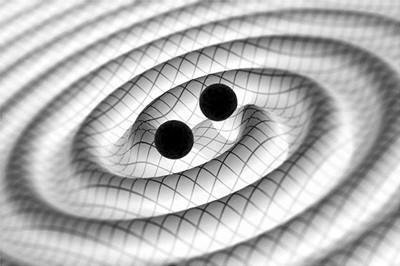
\includegraphics[scale=0.35]{img/gravitational-wave}
 \caption{双黑洞合并过程中产生引力波示意。}
 \label{fig:gravitational-wave}
\end{figure}

\index{音程}
2500年前,正是追寻天籁之音的过程,使得古希腊的先贤毕达哥拉斯发现了音乐背后的数学秘密。相传有一天毕达哥拉斯经过铁匠铺,听到从里面传出了悦耳的声音。这些声音是铁匠们用不同重量的铁锤一起敲打铁砧时产生的。巴洛克时期的音乐家亨德尔有一部作品叫做《快乐的铁匠》(作品编号:HWV430)。毕达哥拉斯注意到有些声音是和谐的,而另一些不和谐。他进一步发现当铁锤的重量比恰好是12、9、8、6时,敲打的声音是和谐的。毕达哥拉斯敏锐地发现了音乐背后的数字规律:

\begin{itemize}
\item 比例$12:6$(即$2:1$)对应纯8度音;
\item 比例$9:6$(即$3:2$)对应纯5度音;
\item 比例$12:9$(即$4:3$)对应纯4度音;
\item 比例$9:8$对应纯2度音。
\end{itemize}

%% \begin{figure}[htbp]
%%  \centering
%%  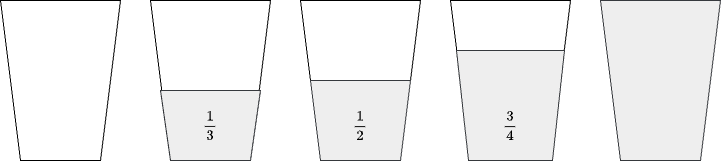
\includegraphics[scale=0.4]{img/cups}
%%  \caption{盛有不同水的杯子}
%%  \label{fig:fraction-cups}
%% \end{figure}

这个故事非常流行,如\ref{fig:pythagoras-music}所示。这幅四联木刻连环画展示了毕达哥拉斯先是聆听到铁匠们挥舞铁锤敲打,然后他开始进行\underdot{定量}研究,包括敲打不同重量的钟,敲打盛有不同水的杯子,弹拨坠有不同重量的琴弦,吹奏不同长度的笛子。但这个故事经不起推敲,第二幅图和第一幅图是相互矛盾的。我们可以自己动手验证一下。依照第二幅图中的样子,用几个同样的杯子盛上不同的水,然后用不同大小的勺子敲击。我们会发现音调的高低是由杯子而不是勺子决定的。同理,铁匠铺传出的音调高低是由铁砧而不是锤子决定的。但第一幅图中只有一个铁砧。这组连环画还有别的问题。铁锤、钟、杯子、琴弦上的砝码、笛子上的数字4、6、8、9、12、16是印度——阿拉伯数字(见第\ref{sec:hindu-arabic-numerals}节),要到十三、十四世纪才传入欧洲。古希腊的毕达哥拉斯不可能用这样的数字。尽管如此,这组连环画仍然反映了毕达哥拉斯求知好学,善于思考,动手实践进行定量研究的治学传统。

\begin{figure}[htbp]
 \centering
 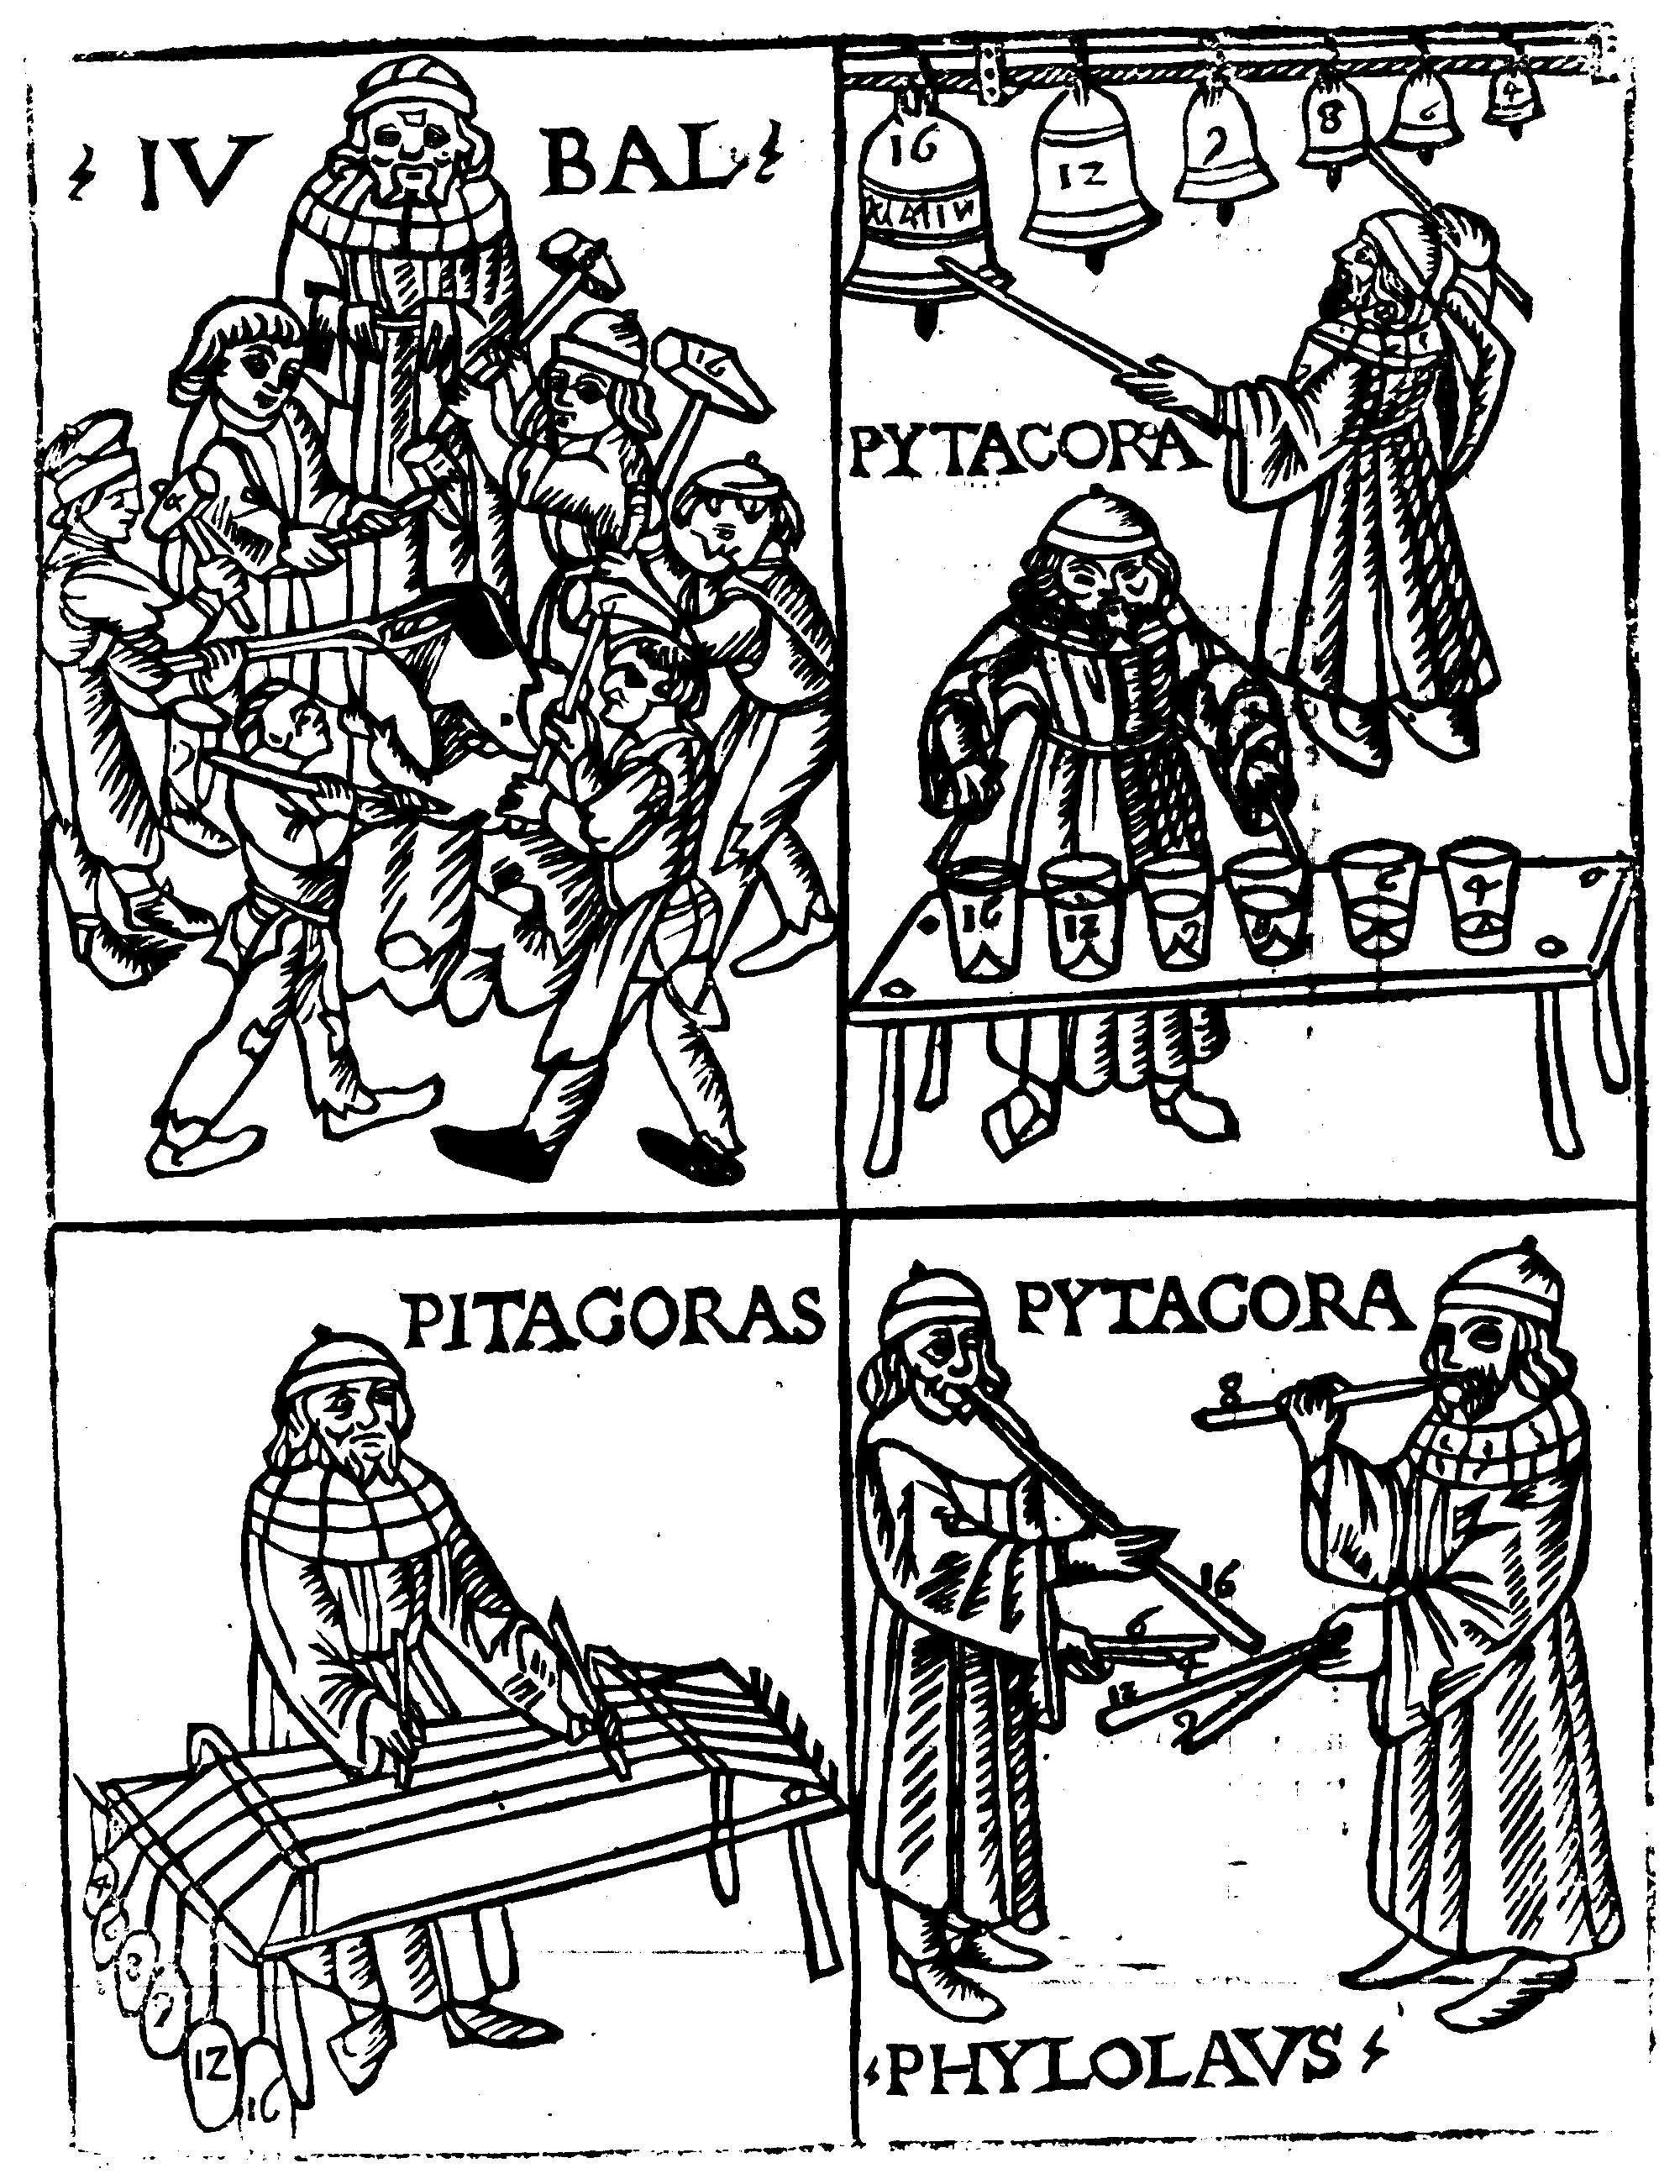
\includegraphics[scale=0.1]{img/pythagoras-music}
 \caption{毕达哥拉斯与音乐,出自1492年(或1480年)弗兰奇诺・加富里奥《乐理》中的木刻插页。}
 %% Woodcut showing Pythagoras with bells, a kind of glass harmonica, a monochord and (organ?) pipes in Pythagorean tuning. From Theorica musicae by Franchino Gaffurio, 1492 (1480?)
 %% https://commons.wikimedia.org/wiki/File:Gaffurio_Pythagoras.png
 \label{fig:pythagoras-music}
\end{figure}

\index{里尔琴}
古希腊的乐器叫做里尔琴(Lyre,也译作里拉琴、莱雅琴、诗琴),是一种七弦琴(见\cref{fig:lyre}),在很多场合已经成为代表音乐的符号。我们推测毕达哥拉斯把琴弦的一半,也就是$\frac{1}{2}$张紧弹奏,获得了8度音;把琴弦的$\frac{2}{3}$张紧弹奏,获得了5度音;把琴弦的$\frac{3}{4}$张紧弹奏,获得了4度音;这些音调之间的关系如\cref{fig:octave}所示。

\begin{figure}[htbp]
 \centering
 \subcaptionbox{绘有太阳神阿波罗手持里尔琴的盘子,约公元前480~470年,藏于雅典德尔菲博物馆。\label{fig:lyre}}{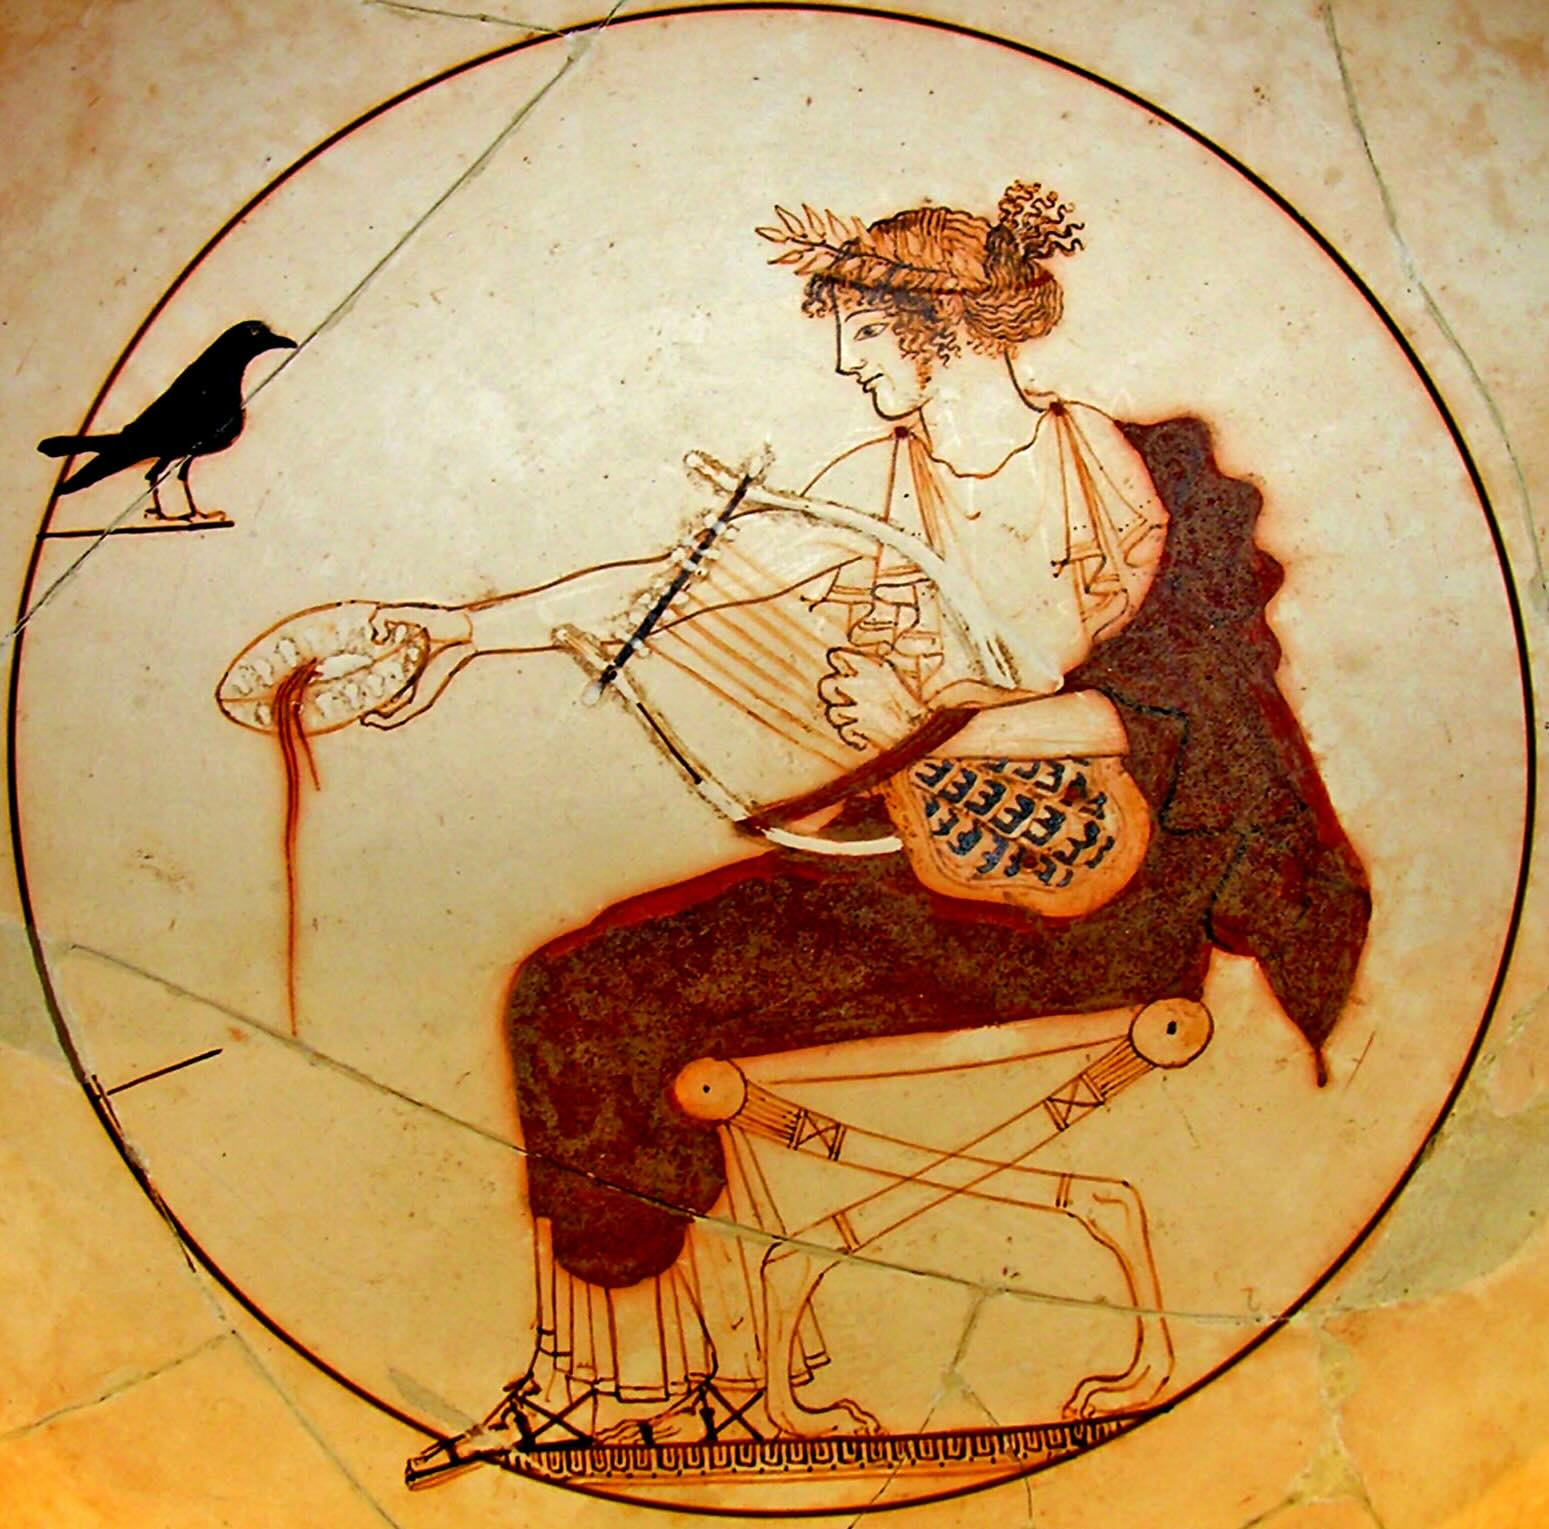
\includegraphics[scale=0.4]{img/apollo-with-lyre}}
 \subcaptionbox{里尔琴符号}{
\includegraphics[scale=0.35]{img/lyre-icon}}
 %% https://www.worldhistory.org/image/986/apollo-with-lyre/
\end{figure}

毕达哥拉斯通过数学,具体说是\underdot{分数与比例}奠定了西方音乐的理论基础。他认为整个宇宙是一把巨大的里尔琴,古希腊人所知道的七个天体(日月和五大行星水星、金星、火星、木星、土星)是琴上的七根弦,在不同的音调上震动。而数与比例代表着宇宙和谐的天籁之音。

\begin{figure}[htbp]
 \centering
 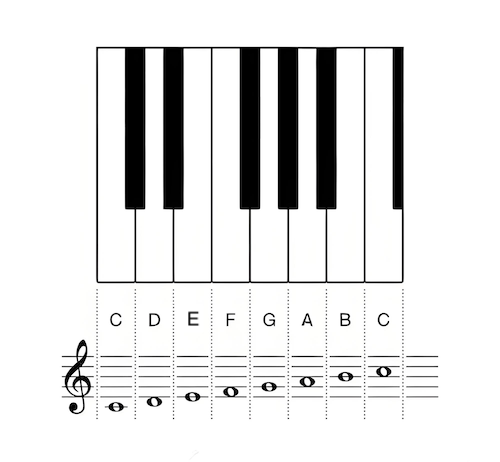
\includegraphics[scale=0.4]{img/octave}
 \caption{两个C间隔8度,琴弦比$2:1$;C与G间隔5度,琴弦比$3:2$;C与F间隔4度,琴弦比$4:3$。}
 \label{fig:octave}
\end{figure}

分数的历史比零和负数还要长。古代中国在春秋时代(公元前770年~前476年)的《左传》中,规定了诸侯的都城大小:最大不可超过周文王国都的三分之一,中等的不可超过五分之一,小的不可超过九分之一。但它们只是表达某种部分的量的词语,而不是真正意义上的分数,因为它们没有直接参与加减乘除运算。清华大学收藏的战国中晚期(最晚公元前305年前后)的楚简中有一个《算表》可以方便地计算99以内的乘法。其中有专门计算乘以二分之一的行和列,对应算出了$\frac{1}{4}, \frac{1}{2}, 1\frac{1}{2}, 2\frac{1}{2}, \dotsc, 4\frac{1}{2}$的结果\citepage[20-22页]{CaoNa-2017}。古代中国到汉代已发展出了完整的分数计算规则,见\ref{sec:chinese-fractions}节。最早的分数出现在古埃及。

\section{埃及分数}
\index{纸草书}
我们是通过两份重要的古代文件了解到埃及分数的。它们是莱茵德纸草书(见\cref{fig:rhind-papyrus})和莫斯科纸草书(见\cref{fig:moscow-papyrus})。所谓纸草书\footnote{英文Papyrus,是纸的英文paper的字源}是古埃及广泛使用的书写载体。它用当时盛产于尼罗河三角洲的纸莎草的茎作为材料,经过切片、浸泡、压制、干燥制成。在公元前3000年左右甚至出口到希腊。莎草纸在埃及的干燥气候下可以很好地保存,经历千年而不腐坏。但在潮湿的环境下,很容易霉变损毁。这两份保留了古埃及数学成果的纸草书异常珍贵。它们一份由英国埃及学者莱茵德(Rhind)于1858年购得,现藏于大英博物馆。内容是公元前1650年前后的教科书,作者是书记官阿梅斯\footnote{Ahmes,也译作阿默斯。},包含有85道数学问题。莫斯科纸草书又名戈列尼雪夫纸草书,由俄罗斯贵族戈列尼雪夫于1893年在埃及购得,现藏于莫斯科普希金精细艺术博物馆。作者是约公元前1890年的一位佚名作者,包含有25道数学问题。

\begin{figure}[htbp]
 \centering
 \subcaptionbox{莱茵德纸草书局部\label{fig:rhind-papyrus}}{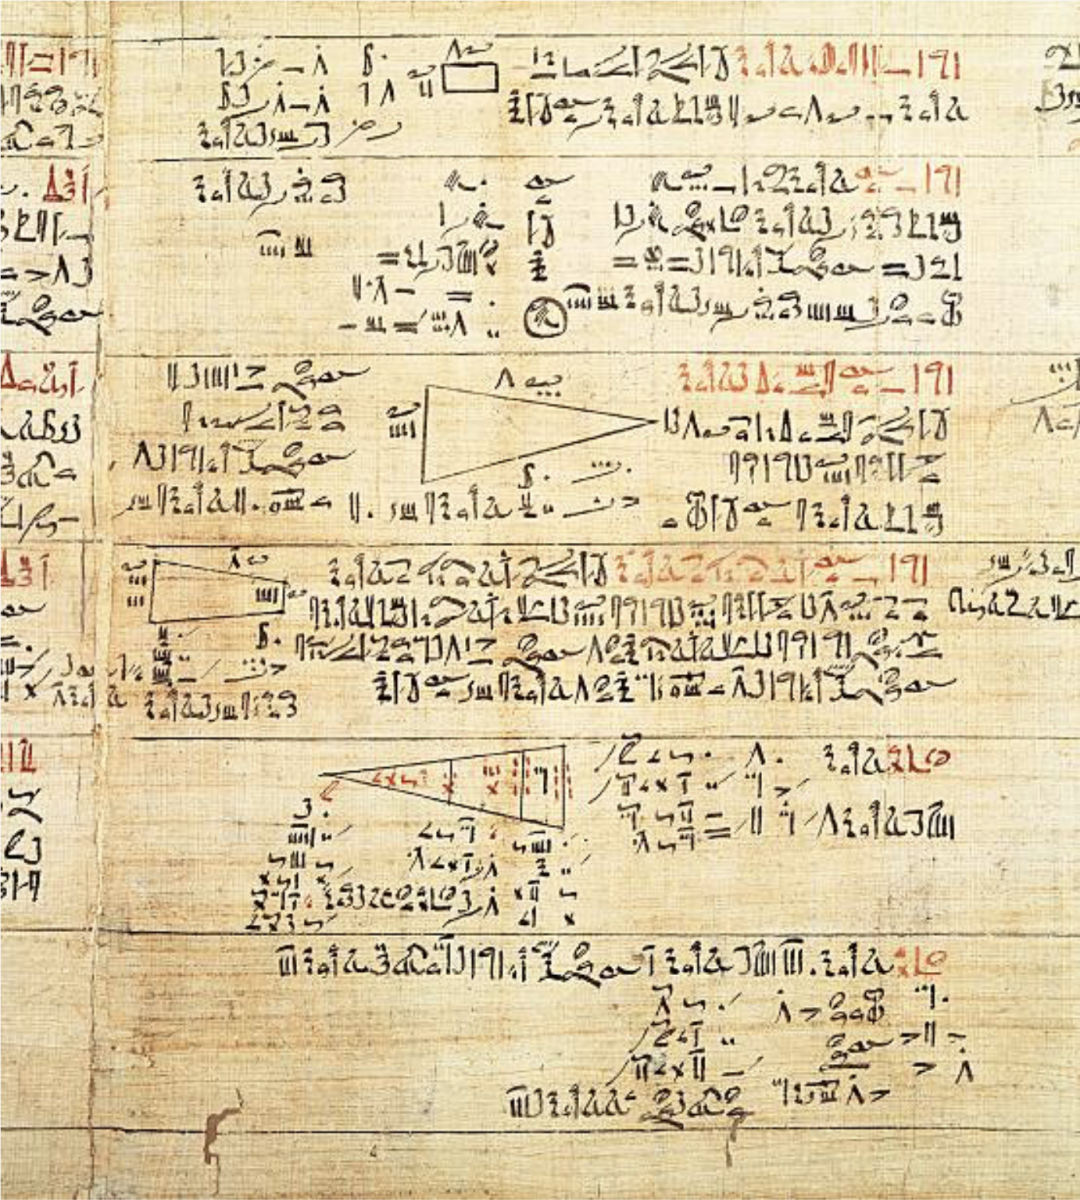
\includegraphics[scale=0.2]{img/rhind-papyrus-part}} \quad
 \subcaptionbox{莫斯科纸草书局部\label{fig:moscow-papyrus}}{ 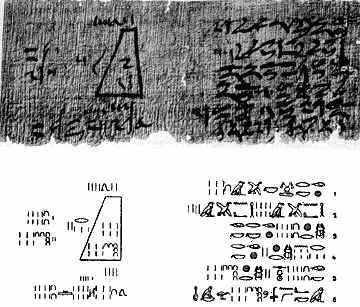
\includegraphics[scale=0.4]{img/moscow-papyrus}}
 %% https://www.britishmuseum.org/collection/image/366139001
 %% https://old.maa.org/press/periodicals/convergence/mathematical-treasure-the-rhind-and-moscow-mathematical-papyri
 %% https://mathshistory.st-andrews.ac.uk/HistTopics/Egyptian_papyri/
\end{figure}

\index{埃及分数}
这两份文物反映了古埃及人已使用分数参与运算解决问题。但古埃及的分数有一个既奇怪又合理的特点——所有的分子都是1。因此被称为“单位分数”。在古埃及象形文字(圣书体,见\ref{sec:rosetta-stone}节)中,在数字$a$上方写(画)一个“眼睛”来表示$\frac{1}{a}$,如所\cref{fig:egyptian-fractions}示,表示$\frac{1}{5}$和$\frac{1}{15}$。单位分数的意义是直观易懂的。$\frac{1}{3}$表示把某物均分3份后每份的量,$\frac{1}{5}$是均分5份后每份的量,$\frac{1}{a}$是均分$a$份后每份的量。

\begin{figure}[htbp]
 \centering
 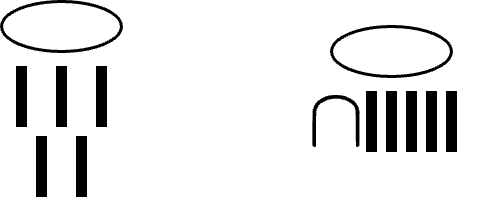
\includegraphics[scale=0.3]{img/egyptian-fractions}
 \caption{埃及分数$\frac{1}{5}$和$\frac{1}{15}$}
 \label{fig:egyptian-fractions}
\end{figure}

但是$\frac{3}{4}$、$\frac{2}{7}$这样的值分子不为1,古埃及人就把它们表示为单位分数之和。例如$\frac{3}{4} = \frac{1}{2} + \frac{1}{4}$,写成象形文字如\cref{fig:sum-egyptian-fractions}左侧所示。中间的符号象征着一个人行走的双腿。如果行走的方向同书写方向一致表示相加,行走的方向同书写的方向相反表示相减。\cref{fig:sum-egyptian-fractions}右侧表示$\frac{2}{5} (= \frac{1}{3} + \frac{1}{15})$。将一个值表示为单位分数的和时,古埃及人要求每个单位分数都不同,不允许重复。因此$\frac{2}{7}$不能写成$\frac{1}{7} + \frac{1}{7}$而要写成$\frac{1}{4} + \frac{1}{28}$。某些情况下,仅仅分解为两个单位分数是不够的。例如莱茵德纸草书上将$\frac{2}{29}$分解为$\frac{2}{29} = \frac{1}{24} + \frac{1}{58} + \frac{1}{174} + \frac{1}{232}$。并且分解方式是不唯一的,例如$\frac{2}{29} = \frac{1}{15} + \frac{1}{435} = \frac{1}{16} + \frac{1}{232} + \frac{1}{464}$。这样的分解没有明显的规律,普通人难以掌握。为此,古埃及人制作了大量的表格以供查找计算。

\begin{figure}[htbp]
 \centering
 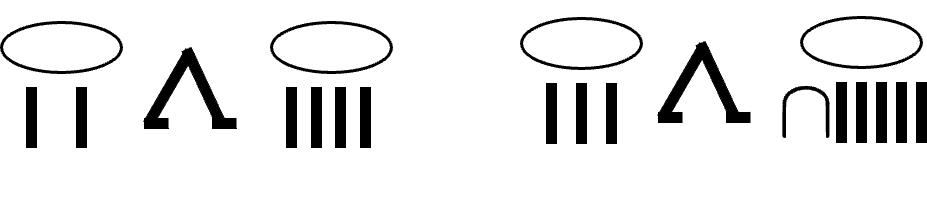
\includegraphics[scale=0.3]{img/sum-egyptian-fractions}
 \caption{左:$\frac{1}{2} + \frac{1}{4}$ \qquad 右:$\frac{1}{3} + \frac{1}{15}$}
 \label{fig:sum-egyptian-fractions}
\end{figure}

迄今为止,没有发现直接的文献,揭示为何古埃及人将分数系统设计为不同的单位分数之和。我们只能加以猜测。有一则传说故事说:老父亲在临终前希望把自己的遗产分给三个儿子。给大儿子$\frac{1}{2}$,二儿子$\frac{1}{3}$,小儿子$\frac{1}{9}$。但全部遗产只是17匹马。三个儿子不知道如何分配,也不愿杀死马进行分割。他们于是去请教村里的长者。老人将自己的一匹马借给了他们。于是大儿子分得$18 \times \frac{1}{2} = 9$匹马,二儿子分得$18 \times \frac{1}{3} = 6$匹马,小儿子分得$18 \times \frac{1}{9} = 2$匹马,剩余$18 - 9 - 6 - 2 = 1$匹马,恰好就是智慧的老人借给他们的那一匹。于是物归原主,老人牵走了他自己的马。这个传说故事用埃及分数解释就是

\[
\frac{17}{18} = \frac{1}{2} + \frac{1}{3} + \frac{1}{9}
\]

尽管脍炙人口,这个传说\underdot{不可能}是古埃及人发展分数系统的初衷。我们在各个民族,包括阿拉伯、印度、犹太、中国的民间故事中都发现了类似的故事。分配的遗产有马、骆驼、大象等动物,数量也有不同。例如三个儿子按照$\frac{1}{2}$、$\frac{1}{4}$、$\frac{1}{6}$分配11个动物,体现为:

\[
\frac{11}{12} = \frac{1}{2} + \frac{1}{4} + \frac{1}{6}
\]

\cref{qn:three-sons}要求给出所有能这样进行分配的数量和比例。我们最早在十八世纪伊朗哲学家纳拉奇(Mulla Muhammad Mahdi Naraqi)的著作中看到此故事的文字记载。其次,尽管在莱茵德纸草书中有关于遗产分配的问题,但主要的分数应用是平均分配。例如第63题\citepage[15页]{MKlein-1972}:把700块面包分给四个人,第一人得$\frac{2}{3}$,第二人得$\frac{1}{2}$,第三人得$\frac{1}{3}$,第四人得$\frac{1}{4}$。阿梅斯的解法在我们今天看来相当于解方程\footnote{$\frac{2}{3}$是古埃及极少数特殊的量,不需要写成单位分数之和。}:

\[
\frac{2}{3}x + \frac{1}{2}x + \frac{1}{3}x + \frac{1}{4}x = 700
\]

他把$\frac{2}{3}$、$\frac{1}{2}$ 、$\frac{1}{3}$ 、$\frac{1}{4}$加起来得到$1\frac{3}{4} (= 1 + \frac{1}{2} + \frac{1}{4})$,然后用1除以$1\frac{3}{4}$得$\frac{4}{7} = (\frac{1}{2} + \frac{1}{14})$。最后$700 \times \frac{4}{7} = 400$,从而得到$x = 400$。这相当于我们今天小学高年级的一元一次方程。注意到第一个人和第三个人分得的面包不是整数块。

另一种观点认为,这种分数系统可以用更经济的方式分配物品。考虑将5块面包分给8个人。一种方法是将每个面包平均切分成8份,然后每人拿5块,如\cref{fig:evenly-devide}所示。

\begin{figure}[htbp]
 \centering
 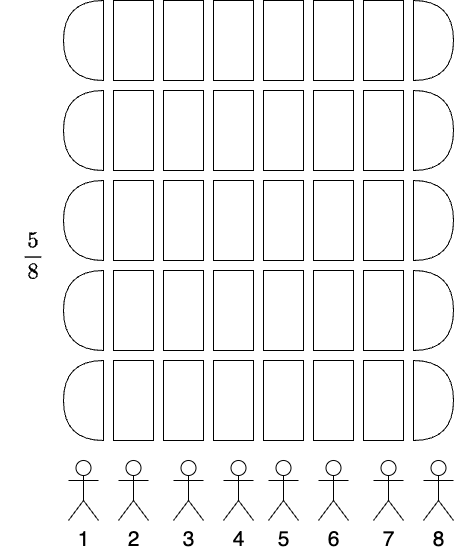
\includegraphics[scale=0.3]{img/evenly-divide}
 \caption{共切成了40小块,每人分得5块。}
 \label{fig:evenly-devide}
\end{figure}

古埃及人可能发现了更好的切割方式,如\cref{fig:egyptian-devide}所示。即每个人拿走半块面包和$\frac{1}{8}$面包。

\begin{figure}[htbp]
 \centering
 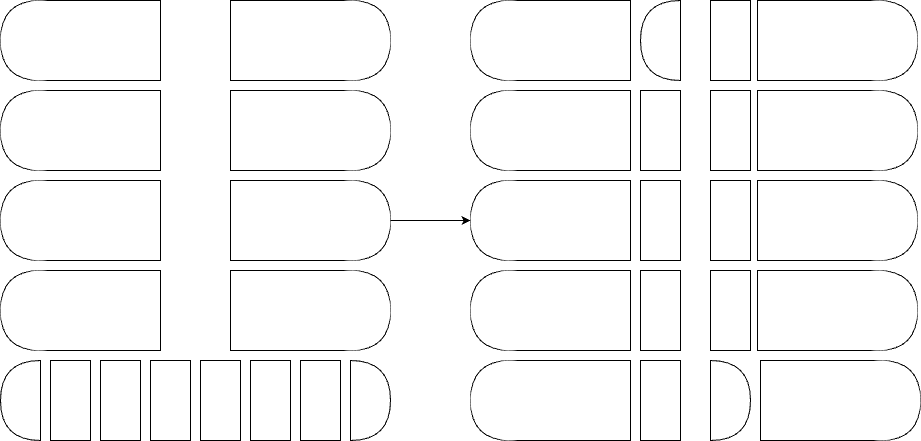
\includegraphics[scale=0.3]{img/egyptian-divide}
 \caption{共切成了16块,每人分得2块(一大$\frac{1}{2}$和一小$\frac{1}{8}$)。}
 \label{fig:egyptian-devide}
\end{figure}

读者朋友们,你觉得古埃及人为何如此设计他们的分数系统呢?以后来的眼光来看埃及分数,一方面它的计算很复杂,逐渐被历史的长河淘汰了,另一方面,数学家思考这样的问题:1)是否每个分数都可以分解成埃及分数?2)如果可以分解,怎样的分解方式最好?其中第一个问题在1202年由斐波那契在《算盘书》中解决了。而第二个问题催生了至今仍未解决的数学猜想。在此之前,我们先看两个相对简单的问题。

\index{埃及分数!分解}
\begin{proposition}每个埃及分数都可以分解为两个不同的埃及分数之和,即$\dfrac{1}{n} = \dfrac{1}{a} + \dfrac{1}{b}$。\label{th:egyptian-fraction-split}
\end{proposition}

\begin{proof}
  \begin{align*}
    \frac{1}{n} &= \frac{n+1}{n(n+1)} & \text{上下同}\times (n + 1) & \\
                &= \frac{\cancel{n}}{\cancel{n}(n+1)} + \frac{1}{n(n+1)} && \\
                &= \frac{1}{n+1} + \frac{1}{n(n+1)} && \qedhere
  \end{align*}
\end{proof}

我们可以立即用这个结论推出:

\begin{proposition}
每个$\dfrac{2}{n}$都能分解为埃及分数。\label{th:decompose-of-2-n}
\end{proposition}

\begin{proof}
  \begin{align*}
    \frac{2}{n} &= \frac{1}{n} + \frac{1}{n} && \\
                &= \frac{1}{n} + \frac{1}{n+1} + \frac{1}{n(n+1)} & \text{上面证明的结论} & \qedhere
  \end{align*}
\end{proof}

当$n$是奇数时,我们能得到更好的结果:$\dfrac{2}{n}$一定能分解为两个埃及分数:

\begin{proof}
  \begin{align*}
    \frac{1}{n} &= \frac{1}{n+1} + \frac{1}{n(n+1)} & \text{由命题\ref{th:egyptian-fraction-split}} & \\
    \frac{2}{n} &= \frac{2}{n+1} + \frac{2}{n(n+1)} & \text{左右同} \times 2 & \\
                &= \frac{1}{\frac{1}{2}(n+1)} + \frac{1}{n\frac{1}{2}(n+1)} & n\text{是奇数,上下同} \div 2 &\qedhere
  \end{align*}
\end{proof}

进一步,\cref{qn:unique-decompose-r}要求证明当$n$是奇素数时,这种分解是唯一的。莱茵德纸草书中有一张表记录了从$\frac{2}{5}$到$\frac{2}{101}$的所有分解,印证了这个结论。回到斐波那契证明的定理,考虑任何即约分数\footnote{分子、分母不能进一步约分的分数。顾名思义,“即约”指完成了约分。}。如果它是假分数,可以先转化成带分数,然后只考虑分解真分数部分。所以只需要证明:

\index{斐波那契定理}
\begin{theorem}[斐波那契]
任何即约真分数$\dfrac{b}{a}$可分解为埃及分数。
\end{theorem}

\begin{proof}
斐波那契利用带余数的除法:$a = bq + r$,其中$q$是商\footnote{《说文解字》:商,从外知内也。汉《律历志》云:商之为言章也,物成熟,可章度也。《白虎通》:章其远近,度其有亡。度量的涵义引申为除法中的商。}、$r$是余数,且$0 < r < b$。最接近并小于$\frac{b}{a}$的分数是$\frac{1}{q + 1}$。斐波那契考虑
\[
  \frac{b}{a} = \frac{1}{q + 1} + x
\]
然后再把$x$分解为埃及分数。通过这一分而治之的思想,原来的问题就转化为分解$x$的问题。
\begin{align*}
  x & = \frac{b}{a} - \frac{1}{q + 1} = \frac{bq + b - a}{a(q + 1)} & \text{通分} \\
    & = \frac{b - (a - bq)}{a(q+1)} = \frac{b - r}{a(q+1)} & \text{余数}r = a - bq
\end{align*}
注意到$x$的分子$b' = b - r$。由于余数$0 < r < b$,所以$b' < b$,它比原分数$\frac{b}{a}$的分子$b$至少减小了1。如果$b' = 1$,则分解完成,否则我们继续分解$x$。这样就可以得到一系列不断缩小的分子序列$b > b' > b'' > \cdots$因为$b$是一个确定的正整数,它不会无限减小,所以必定在某次达到1从而结束分解。因此每个即约真分数都可以分解为埃及分数。
\end{proof}

我们用一个例子$\frac{5}{11}$来理解斐波那契的证明。$11 = 2 \times 5 + 1$,商$q = 2$、余数$r = 1$。第一步分解:

\begin{align*}
\frac{5}{11} & = \frac{1}{q + 1} + x = \frac{1}{3} + x  \\
 x &= \frac{5}{11} - \frac{1}{3} = \frac{4}{33} \\
\frac{5}{11} &= \frac{1}{3} + \frac{4}{33}
\end{align*}

接下来分解$\frac{4}{33}$。再次用带余数除法$33 = 4 \times 8 + 1$,商$q = 8$、余数$r = 1$。

\begin{align*}
\frac{4}{33} & = \frac{1}{q + 1} + x = \frac{1}{9} + x  \\
 x &= \frac{4}{33} - \frac{1}{9} = \frac{12 - 11}{99} = \frac{1}{9}
\end{align*}

分解结束,得到:
\[
\frac{5}{11} = \frac{1}{3} + \frac{1}{9} + \frac{1}{99}
\]

\index{贪心策略}
斐波那契使用的策略是每次用\underdot{最接近}原分数$\frac{b}{a}$的埃及分数进行分解。这种策略叫做\underdot{贪心策略}。但是贪心策略并不一定给出最优分解。例如

\[
\frac{5}{121} = \frac{1}{25} + \frac{1}{757} + \frac{1}{763309} + \frac{1}{873960180913} + \frac{1}{1527612795642093418846225}
\]

但还有另一个分解:
\[
\frac{5}{121} = \frac{1}{33} + \frac{1}{121} + \frac{1}{363}
\]

所谓最优的含义是:用\underdot{最少}的埃及分数分解,如果两个分解的埃及分数个数相同,则分母越小越好。
附录\ref{app:best-egyptian-decomposition}介绍了一个寻找最优分解的算法。
斐波那契的方法每次至少将分子减1,所以$\frac{b}{a}$最多一定被分解为$b$个埃及分数,但$\frac{5}{121}$的例子说明可能存在着更好的分解方法。匈牙利数学家保罗·埃尔德什和德国数学家斯特劳斯在1950年猜想对于大于1的自然数$n$,\index{埃尔德什——斯特劳斯猜想}

\[
\frac{4}{n} = \frac{1}{a} + \frac{1}{b} + \frac{1}{c}
\]
总成立,其中$a < b < c$。也就是说$\frac{4}{n}$总能分解为3个两两不同的埃及分数。这个著名的数论问题称为埃尔德什——斯特劳斯猜想\footnote{Erdős - Straus},迄今(2025)仍未解决。
% https://mathworld.wolfram.com/Erdos-StrausConjecture.html

\begin{mdframed}

\begin{center}
 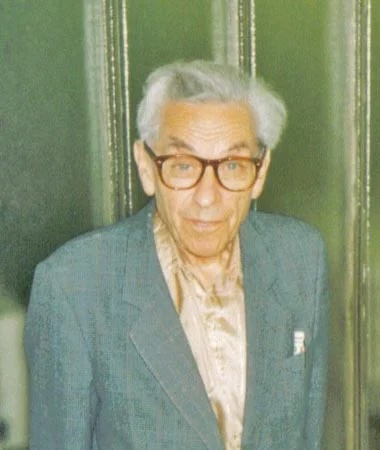
\includegraphics[scale=0.3]{img/erdos-1992}
 \captionof{figure}{保罗·埃尔德什(1913~1996)}
 \label{fig:erdos-1992}
\end{center}

\index{数学家!埃尔德什} \label{sec:Erdos}
保罗·埃尔德什(Paul Erdős),匈牙利籍犹太人,著名的“自由职业”数学家。一生发表论文1500多篇(包括与其他作者合作),是迄今发表论文数最多的数学家(第二位为欧拉)。埃尔德什在数论、组合数学等方面作出了很大贡献\cite{Hoffman-Paul-2025}。他四处游历,探访当地的数学家,与他们一起工作,曾和507人合写论文\footnotemark。这使得他事实上成为了一个巨大的数学合作网络的中心人物。因此有人定义了“埃尔德什数”,简称埃数。埃尔德什自己的埃数为0,与他直接合作写论文的人的埃数为1,与埃数为1的人合写论文的人埃数为2,依此类推。例如爱因斯坦的埃数为2,菲尔兹奖获奖者的埃数中值最低时为3。目前已知最大的埃数为15(不包括非数学家,他们的埃数为无穷大)。

%% 例如 https://www.jmilne.org/math/Personal/index.html 页面底部的埃尔德什数

1913年,埃尔德什出生在匈牙利首都布达佩斯,父母都是犹太人。埃尔德什出生前两个姐姐都死于可怕的猩红热,父母生怕他夭折,因此对他格外呵护。可是生逢乱世,他还不到1岁第一次世界大战就爆发了。父亲在沙俄与奥匈帝国的战争中被俘,被关在西伯利亚的战俘营6年直至战争结束才生还。令人惊讶的是,埃尔德什的父亲在被俘期间自学了英语。由于没有人教授发音,父亲读音很奇怪。埃尔德什从他父亲那里也学到了这种奇怪的口音,并持续终生。一战后的匈牙利政局混乱,罢工不断。作为中学数学教师的母亲为了不影响孩子们的教育坚持上课,结果政局变乱时,她因不参与罢工而丢掉了工作。1920年匈牙利已经开始迫害犹太人,13年后希特勒上台,欧洲进一步走向了战争。

尽管环境如此恶劣,埃尔德什在匈牙利全国考试中脱颖而出,考入了布达佩斯的帕兹马尼・彼得大学,并于1934年获得了博士学位。可是犹太人的处境恶劣,他选择了去英国曼彻斯特大学做博士后研究。在剑桥大学,他认识了数学家哈代和乌拉姆,后者成了他的终身朋友。埃尔德什想探望在匈牙利的父母,但希特勒在1938年占领了奥地利和捷克,他被迫在中途逃回,并辗转到了美国普林斯屯高等研究院。埃尔德什花了1年时间与他人合作创立了概率数论,但研究院不知为何
%%看不上这位只有25岁的年轻人,--此说恐怕不妥
只答应延长6个月任期。乌拉姆在这个困难的时候伸出援手,邀请埃尔德什去麦迪逊的威斯康星大学。这开启了埃尔德什四处游历,随遇而安研究数学的“流浪生活”。

埃尔德什坚信上帝手中有一本“天书”,里面包含着最优美、最简洁的数学证明。他毕生都在追寻那些“数学天书中的证明”。尽管有些定理已经被证明了,埃尔德什会继续寻找更完美,有时甚至是初等的证明。比如1845年约瑟夫·伯特兰猜想任何整数$n$和$2n$之间至少存在着一个素数。1850年切比雪夫证明了这个猜想,因此今天它叫做“波特兰——切比雪夫定理”。埃尔德什在19岁时重新用初等方法证明了这个猜想。他对自己的证明很满意,相信这就是“天书”中的证明。“这简直来自数学天书!”成了埃尔德什对他人工作的最高评价。1998年,埃尔德什诞生85周年之际,数学家们收集了最优美的45个证明汇集成了一本《数学天书中的证明》。

第二次世界大战中,埃尔德什和匈牙利的家人完全失去了联系。战争结束后他才获知,父亲已经于1942年因心脏病突发去世。家里有4位亲属被害,有位表兄弟是奥斯维辛集中营的幸存者。最幸运的是,母亲还活着。从1943年起,埃尔德什“云游”在普渡大学、斯坦福大学、圣母大学、约翰斯·霍普金斯大学之间。他没有全职教职,但反而可以自由选择和任何人合作研究任何喜欢的问题。这种生活即工作,工作即生活的人生持续了半个世纪。居无定所、没有妻子、没有孩子、没有固定工作的羁绊。足迹遍布22个国家,尽管有时不得不在某些国境线前返回:冷战期间,他的祖国匈牙利怀疑他是间谍而拒绝其入境。美国在麦卡锡主义盛行时也禁止他入境。尽管没有披露原因,有人猜测他与1949年回国的中国数学家华罗庚在通信中讨论数学问题,移民局的官员们担心信中那些宛如天书的数学符号可能是密码……\cite{MacTutor-Erdos-2000}不速之客埃尔德什经常突然出现在某位数学家的门口:“我的大脑敞开了!”然后住在别人家里一段时间,一起研究有趣的数学问题。

埃尔德什是匈牙利科学院、美国科学院、英国皇家学会会员。他在1951年获得科尔奖,在1984年获得沃尔夫奖。面对5万美元奖金,他只花掉了720美元,而把剩下的全部捐出设立奖学金以纪念他的父母。1996年,83岁的埃尔德什在波兰华沙突发心脏病去世。在几个小时前,他刚刚在华沙的学术会议上解决了一个棘手的几何问题。

\end{mdframed}
\footnotetext{一说为511人。在埃尔德什死后,仍有70多篇以他为作者的论文发表\citepage[588页]{Stillwell-2010}。}

\section{古巴比伦的分数}
以今天的眼光来看,埃及分数不便于计算,像是在数学上走了一段弯路。它的形式意义大于它的实用意义。此后的古希腊、古罗马并未发展出独立的分数系统,而是用一些特定的词汇表示部分的量。古罗马表示部分的词汇来源于其重量单位系统。单位重量叫做as,它的$\frac{1}{12}$叫做uncia,是英制重量盎司ounce的词源。\cref{tab:roman-fractions}列出了常用的罗马分数名词:
\index{罗马分数}

% https://mathshistory.st-andrews.ac.uk/Miller/mathsym/fractions/
\begin{table}
  \centering
  \begin{tabular}{|c|l|l||c|l|l|}
  \hline
  值 & 词汇 & 意义 & 值 & 词汇 & 意义 \\
  \hline
  $\frac{1}{12}$ & uncia    & 十二分之一 & $\frac{9}{12}$ & dodrans    & 去掉四分之一 \\
  \hline
  $\frac{2}{12}$ & sextans  & 六分之一 & $\frac{10}{12}$ & dextans   & 去掉六分之一 \\
  \hline
  $\frac{3}{12}$ & quadrans & 四分之一 & $\frac{11}{12}$ & deunx    & 去掉一个uncia \\
  \hline
  $\frac{4}{12}$ & triens   & 三分之一 & $\frac{1}{24}$ & semuncia   & uncia的一半  \\
  \hline
  $\frac{5}{12}$ & quincunx & 五个uncia & $\frac{1}{48}$ & sicilicus &  \\
  \hline
  $\frac{6}{12}$ & semis    & 一半    & $\frac{1}{72}$ & scriptulum    &  \\
  \hline
  $\frac{7}{12}$ & septunx  & 七个uncia & $\frac{1}{144}$ & scripulum  &  $\frac{1}{12} \times \frac{1}{12}$ \\
  \hline
  $\frac{8}{12}$ & bes      & 三分之二 & $\frac{1}{288}$ & scrupulum    &  $\frac{1}{24} \times \frac{1}{12}$\\
  \hline
  \end{tabular}
  \caption{罗马分数名称}
  \label{tab:roman-fractions}
\end{table}

有许多词至今仍影响着我们的语言。表示$\frac{1}{2}$的semi,常用作“半”的词根,例如半圆semicircle、分号semicolon、半导体semiconductor等。表示$\frac{1}{4} = \frac{3}{12}$的quadrans在英语中是quarter,仍表示一刻钟、一季度。

\index{古巴比伦小数}
古巴比伦发展出了分数系统。我们从耶鲁大学收藏的一块泥板中找到了“物证”,如\cref{fig:babylonian-yale}所示。此图描绘了一个正方形和对角线。正方形的一边刻有楔形文字30(右上角的3个楔形),在对角线下刻有文字42, 25, 35,贯穿着这同一对角线还刻有文字1, 24, 51, 10。我们在初中数学课上学到过正方形的对角线长度是边长的$\sqrt{2}$倍。简单计算$30 \times \sqrt{2} \approx 30 \times 1.4142 = 42.426$,其中42恰好是对角线下所刻文字的第一个。古巴比伦人使用60进制,我们怀疑接下来的25, 35是小数部分。这很容易验证:

\begin{figure}[htbp]
 \centering
 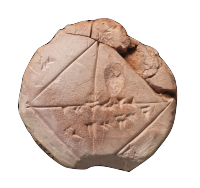
\includegraphics[scale=0.8]{img/babylonian-yale}
 \caption{耶鲁大学古巴比伦泥板,编号Y7289}
 \label{fig:babylonian-yale}
\end{figure}

\[
\frac{25}{60} + \frac{35}{60^2} \approx 0.4264
\]

这说明古巴比伦人正确地计算出了对角线长度。42, 25, 35代表$42.426 \approx 30 \times \sqrt{2}$。那么1, 24, 51, 10会不会也是个小数呢?我们试一试:

\[
1 + \frac{24}{60} + \frac{51}{60^2} + \frac{10}{60^3} \approx 1.414213
\]

竟然是$\sqrt{2}$的小数表示,并且精度达到了百万分位(小数点后6位)!我们由此确知古巴比伦人发展出了60进制小数系统。但由于没有小数点,他们的数字是有歧义的。例如12, 15既可能是$12 \times 60 + 15 = 720$也可能是$12 + \frac{15}{60} = 12.25$。再加上0没有被统一使用,我们只能通过上下文猜测一个数的真正含义。

由于使用60进制,古巴比伦人可以比较精细、准确地表示$\frac{1}{60}$~$\frac{59}{60}$之间的部分量。当使用2到3位60进制小数时,已足够生产、生活、乃至天文观测所需的精度。此外,60的真因数\footnote{除1和$n$以外的因数称$n$的真因数。}足够丰富(包括2, 3, 4, 5, 6, 10, 12, 15, 20, 30),除不尽产生循环小数的机会较少(10进制只有2和5两个真因数,只有少数情况能除尽而不循环,参见\cref{thm:cyclic-decimal})。可能由于这些因素,古巴比伦人只使用60进制小数而没有发展出一般的分数系统。

\section{古代中国的分数}
\label{sec:chinese-fractions}

\index{九章算术}
在汉代的《九章算术》中,已经包含了分数四则运算规则和各种应用题。这些内容集中出现在第一卷“方田”中(见\cref{fig:jiuzhang})。由于篇幅不大,我们不妨一起赏析一下中国古人的智慧。首先是分数的记法。《九章算术》中已经使用了“a分之b”这样的描述,和现代汉语完全一致,如:“十五分之一”。古人用步数表示长度,例如一块田长九步、宽五步。当用分数表示长度时,说“a分步之b”,如:“七分步之四”、“五分步之三”。而在现代汉语中,我们说七分之四步、五分之三步。又如表示金额:“八钱三分钱之一”,可见已经有了带分数的概念。对应现代汉语中的八又三分之一钱。《九章算术》中的分数直接来源于除法,如:“七人卖四马,一人卖七分马之四。”这就是$\frac{4}{7}$的意义。

\begin{figure}[htbp]
 \centering
 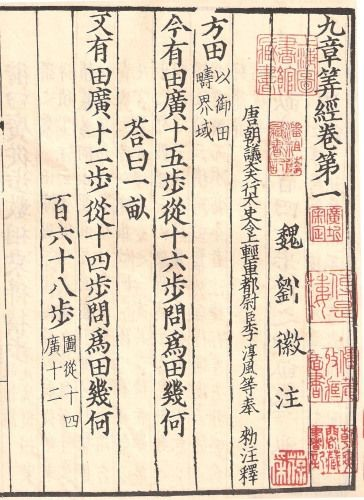
\includegraphics[scale=0.4]{img/jiuzhang}
 \caption{《九章算术》书影}
 \label{fig:jiuzhang} % The Nine Chapters on the Mathematical Art
\end{figure}

\index{约分}
有了分数记法,接下来《九章算术》要处理一个分数的值是否“唯一”的问题。这就引出了“约分”的概念。作者用两道例题说明:
\begin{enumerate}[1)]
\item 今有十八分之十二,问约之得几何?答曰:三分之二。(即:$\frac{12}{18} = \frac{2}{3}$)
\item 又有九十一分之四十九,问约之得几何?答曰:十三分之七。(即:$\frac{49}{91} = \frac{7}{13}$)
\end{enumerate}

\index{辗转相除} \index{欧几里得算法!减法形式} \label{sec:gcd-minus}
具体怎样约分呢?《九章算术》给出了“辗转相除”法,即著名的欧几里得算法求最大公约数(也叫做最大公因数):“可半者半之;不可半者,副置分母、子之数,以少减多,\underdot{更相减损},求其等也。以等数约之。”解释成现代汉语:首先是特殊情况。若分子分母都是偶数,先不断$\div 2$,化为奇数。然后是一般情况。记分数为$\frac{b}{a}$,记$a$与$b$的最大公约数为$(a, b)$,则:

\be
\label{eq:gcd-minus}
(a, b) = \begin{cases}
  a > b :& (a - b, b) \\
  a = b :& a \\
  a < b :& (a, b - a)
  \end{cases}
\ee

就是“以少减多,更相减损、求其等也”的意思。这种方法在欧几里得的《几何原本》中有系统的描述和正确性证明,今天被称做“欧几里得算法”,在中国常被称做辗转相除法。对比一般的方法:把$a$、$b$分解为因子的积,然后找出最多的公因子相乘,欧几里得算法的效率极高\footnote{利用除法代替\cref{eq:gcd-minus}中的减法可以达到“对数复杂度”。100位的整数,大约递归8次左右即可算出。},便于机械化计算,是当今数论和密码学的基础算法\footnote{在抽象代数,如环论、域论中也有重要应用}。我们将在下一章中详细介绍它的原理。这里举一个例子:求18和12的最大公约数。

\[
(18, 12) = (18 - 12, 12) = (6, 12) = (6, 12 - 6) = (6, 6) = 6
\]

只用了3步就求出了结果。最后分子分母同除以最大公约数得:$\frac{12}{18} = \frac{12/6}{18/6} = \frac{2}{3}$。

《九章算术》接下来通过例题引入分数加法:

\begin{enumerate}[1)]
\item 今有三分之一,五分之二,问合之得几何?答曰:十五分之十一。(即:$\frac{1}{3} + \frac{2}{5} = \frac{11}{15}$)
\item 又有三分之二,七分之四,九分之五,问合之得几何?答曰:得一、六十三分之五十。(即:$\frac{2}{3} + \frac{4}{7} + \frac{5}{9} = 1\frac{50}{63}$)
%% \item 又有二分之一,三分之二,四分之三,五分之四,问合之得几何?答曰:得二、六十分之四十三。(即:$\frac{1}{2} + \frac{2}{3} + \frac{3}{4} + \frac{4}{5} = 2\frac{43}{60}$)
\end{enumerate}

作者解释分数加法原理:“母互乘子,并以为实。母相乘为法。”即:

\be
\frac{b}{a} + \frac{d}{c} = \frac{bc + ad}{ac}
\ee

新的分子叫“实”,分母叫“法”。接下来:“实如法而一。不满法者,以法命之。”即$\frac{n}{n} = 1$,抽取整数部分化为带分数。最后说:“其母同者,直相从之。”即:

\be
\frac{b}{a} + \frac{c}{a} = \frac{b + c}{a}
\ee

分母相同时,直接将分子相加。可见《九章算术》的通分并未使用最小公倍数,而是直接将分母相乘。

《九章算术》接下来介绍分数减法,基本上类似于加法,我们省略跳过。之后介绍分数大小的比较。《九章算术》的作者采用和减法一样的处理,通过母子互乘比大小。即将$\frac{b}{a}$与$\frac{d}{c}$的大小比较转化为$bc$与$ad$的大小比较。接下来在介绍多个分数的平均数之后讲解分数除以整数,例如:“今有七人,分八钱三分钱之一。问人得几何?答曰:人得一钱二十一分钱之四。”即$8\frac{1}{3} \div 7 = 1\frac{4}{21}$。作者解释说:“以人数为法,钱数为实,实如法而一。有分者通之。”即用金额作分子,人数作分母。这里并没有考虑除数是分数的情况。最后是分数乘法:

\begin{enumerate}[1)]
\item 今有田广七分步之四,从五分步之三,问为田几何?答曰:三十五分步之十二。(即:$\frac{4}{7} \times \frac{3}{5} = \frac{12}{35}$)
\item 又有田广九分步之七,从十一分步之九,问为田几何?答曰:十一分步之七。(即:$\frac{7}{9} \times \frac{9}{11} = \frac{7}{11}$)
%% \item 又有田广五分步之四,从九分步之五,问为田几何?答曰:九分步之四。(即:$\frac{4}{5} \times \frac{5}{9} = \frac{4}{9}$)
\end{enumerate}

作者给出的计算规则是:“母相乘为法,子相乘为实,实如法而一。”即分子分母相乘再化带分数。有趣的是《九章算术》对带分数乘法进行了单独处理:

\begin{enumerate}[1)]
\item 今有田广三步三分步之一,从五步五分步之二,问为田几何?答曰:十八步。(即:$3\frac{1}{3} \times 5\frac{2}{5} = 18$)
\item 又有田广七步四分步之三,从十五步九分步之五,问为田几何?答曰:一百二十步九分步之五。(即:$7\frac{3}{4} \times 15\frac{5}{9} = 120\frac{5}{9}$)
%% 又有田广十八步七分步之五,从二十三步十一分步之六,问为田几何?答曰:一亩二百步十一分步之七。
\end{enumerate}

作者解释说:“分母各乘其全,分子从之,相乘为实。分母相乘为法。实如法而一。”即化成假分数,相乘再化带分数。例如:

\[
3\frac{1}{3} \times 5\frac{2}{5} = \frac{10}{3} \times \frac{27}{5} = \frac{10 \times 27}{3 \times 5} = 18
\]

《九章算术》一开篇就系统地引入了分数及其四则运算。可见中国古人对分数的重视。后继的各种图形面积、方程计算都建立在这个基础上。

\section{印度分数和小数}

\index{印度分数}
我们今天使用的分数记法源自古印度。印度人将表示分子的数写在上方,将表示分母的数写在下方,但并未使用分数线,如:

\begin{align*}
  3 \\
  4
\end{align*}

\index{分数线}
表示四分之三。后来阿拉伯人在约公元1200年引入了分数线来分开分子与分母\cite{Pumfrey-2011},如:

\[
\dfrac{3}{4}
\]

斐波那契最早将现代分数记法介绍到欧洲,但在写带分数时,他照搬了阿拉伯人从右向左的书写习惯,将分数写在整数的左边\cite{Miller-2025}。分数线带来了不小的印刷困难。在1718年,英国著名的川宁茶叶公司创世人托马斯·川宁\footnote{Thomas Twining}在记账时用斜线代替水平分数线,如:1/4磅茶叶。这样就便于印刷和用打字机书写分数。今天很多字处理和编辑软件可以方便输入分数。不少网页支持了 \LaTeX 排版,可以用\lstinline|\frac{b}{a}|来输入$\frac{b}{a}$。

\index{小数} \index{数学家!刘徽}
随着印度——阿拉伯计数系统的确立,阿拉伯学者开始引入了十进制小数。数学家阿尔·卡西(Al-Kashi,公元920年~980年)在他的著作《圆周的研究》\footnote{{\em al-Risali al-mohitije}译作英文{\em Treatise on the circumference}}中将圆周率$\pi$的值写为:“sah-hah 3 14159”,其中sah-hah的意思是整数部分(今天土耳其语中的sahih),修饰了3,接下来是小数部分。可见此时尚未引入小数点。中国魏晋时的数学家刘徽(见\cref{fig:liuhui})在注解《九章算术》时,不满于古代用3作为圆周率,于是:“微数无名知以为分子,以十为分母”,决定采用十进分数来求得更精确的值。当他用正96边形逼近圆时求得:“三百一十四寸六百二十五分寸之一百六十九”,这个值的表示已经非常接近小数的形式了\footnote{关于这个值,刘徽接着写道:“则出圆之表矣。故还就一百九十二觚之全幂三百一十四寸以为圆幂之定率而弃其余分。”他觉得大了,故得到此时的圆周率3.14。但他不甘心,又继续用192边形计算到“三百一十四寸二十五分寸之四”。这个带分数是$314\frac{4}{25} = 314.16$寸。可见刘徽是混合使用小数和分数的。}。

\begin{figure}[htbp]
 \centering
 \subcaptionbox{纳皮尔肖像,1616年油画,爱丁堡大学收藏\label{fig:napier}}{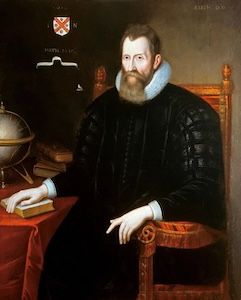
\includegraphics[scale=0.5]{img/napier}} \quad
 % https://www.britannica.com/biography/John-Napier
 \subcaptionbox{蒋兆和创作的刘徽像,部编数学课本\label{fig:liuhui}}{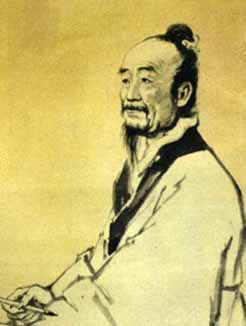
\includegraphics[scale=0.46]{img/liuhui}}
 % https://wapbaike.baidu.com/tashuo/browse/content?id=b1fc49ab180770763a28420d
\end{figure}

\index{小数点} \index{数学家!纳皮尔} \index{百分数}
1530年,鲁道夫(Christoff Rudolff,1499?~1545?年 )使用一条数线分隔整数和小数部分。后来马吉尼(Magini,1555年~1617年)将竖线改进成了小数点,但并未得到广泛使用。直到20年后英国学者约翰·纳皮尔(John Napier,1550年~1617年,见\cref{fig:napier})发明对数时使用了小数点,现代小数形式才被广泛接受。我们常用的百分数符号\%是佚名的某位意大利人在1425年引入的。

\index{基点}
从另一角度看,小数是分母为10、100、1000……的分数的和。百分数看似是分母为100的分数,实则只是小数乘以100的结果。这是因为百分数的分子不一定是整数。例如某网站说它的可靠性非常高,达99.999\%(俗称5个9),这相当于小数0.99999。在日常生活中,人们还会用千分数,写作999.99\textperthousand。在金融领域还会用基点(BPS:base points的缩写)这个量。1bps = 0.01\% = 0.0001。比如我们看见新闻说美联储(美国联邦储备委员会,是美国的中央银行的核心管理机构)宣布降息25个基点。实际上就是降低利息0.25\% = 0.0025。例如利率从2.5\%降低25个基点就变成2.5\% - 0.25\% = 2.25\%。

\subsection{分数与小数的关系}

现在我们回过头来说为何小数是分母为10、100、1000……的分数和?并提出一个问题:是否每个分数都可以\underdot{唯一}地表示成小数?举例来说0.125 = $\frac{1}{10} + \frac{2}{100} + \frac{5}{1000}$,恰好是分母为10的$\frac{1}{10}$,分母为100的$\frac{2}{100}$,分母为1000的$\frac{5}{1000}$的和。一般来说,小数$0.a_1 a_2 \dots a_n$可表示为:

\be
a_1 \frac{1}{10} + a_2 \frac{1}{100} + \cdots + a_n \frac{1}{10^n}
\label{eq:decimal-as-sum}
\ee

\index{无限循环小数}
我们在数学课上知道,小数分为有限小数(如0.125)和无限小数(如$0.\dot{3} = 0.333\cdots, 0.\dot{1}\dot{5} = 0.1515\cdots, \pi = 3.14159\cdots$)。根据\cref{eq:decimal-as-sum},无限小数可写成无限个分数的和。那么这无限个正数的和是个有限值还是无限大?为了解答这个问题,我们先引入一个看似反直觉的命题:

\begin{lemma} \label{th:cycle-of-9}
  无限循环小数$0.999\cdots$的值是1。
\end{lemma}

乍看上去左边的$0.999\cdots$和右边的1明显是两个不同的数,它们怎么会相等呢?

\begin{proof}
  令$x = 0.999\cdots$,扩大10倍:$10x = 9.999\cdots$,相减:
  \begin{align*}
    10x - x &= 9.999\cdots - 0.999\cdots && \\
         9x &= 9 & \text{右侧的小数部分减光了} & \\
          x &= 1  && \qedhere
  \end{align*}
\end{proof}

注意,小数部分只有有限个9时等号不成立,哪怕有$n = 10000$个9。因为$9.99\cdots9$(个位的9和小数部分的9999个9)减$0.99\cdots9$(小数部分的1万个9)等于$8.99\cdots91$。因此$x = \frac{8.99\cdots91}{9} \ne 1$。即1万位有限小数$0.99\cdots9 \ne 1$。这样无限个正数的和$\frac{9}{10} + \frac{9}{100} + \cdots = 1$,是个确定的有限值\footnote{我们也可以用高中数学的极限概念进行证明。注意到$n$位有限小数:$0.99\cdots9 = 1 - 0.00\cdots01 = 1 - \frac{1}{10^{n+1}}$,所以$0.999\cdots = \lim\limits_{n\to\infty} (1 - \frac{1}{10^{n+1}}) = 1 - \lim\limits_{n\to\infty} \frac{1}{10^{n+1}} = 1 - 0 = 1$。}。

\begin{corollary}
  把任何无限小数$0.a_1a_2\cdots$写成无穷多个分数的和:$a_1 \dfrac{1}{10} + a_2 \dfrac{1}{100} + \cdots$这个和是有限的。
\end{corollary}

\begin{proof}
  由于每个小数位$0 \leq a_i \leq 9$,所以
  \begin{align*}
0 \leq 0.a_1 a_2 \cdots = a_1\frac{1}{10} + a_2\frac{1}{10^2} + \cdots \leq \frac{9}{10} + \frac{9}{10^2} + \cdots = 0.999\cdots = 1 & \qedhere
  \end{align*}
\end{proof}

\index{芝诺悖论!阿基里斯与乌龟悖论}
这个结论:$0.a_1a_2\cdots \leq 1$看似说了一句废话,但无限多个(正)值加起来是有限的是一个极为惊人的数学与逻辑断言。它是解决一个有着两千多年历史的悖论的钥匙。古希腊的哲学家,埃利亚的芝诺(Zeno of Elea,约公元前490~425年)提出了著名的四个悖论。第一个悖论最为人们所津津乐道,名叫阿基里斯与乌龟悖论。阿基里斯是荷马史诗《伊里亚特》中的英雄,以英勇著称。这个悖论说:如果让爬得很慢的乌龟在阿基里斯前面一段路程出发,那么阿基里斯将永远追不上乌龟。这是因为,阿基里斯为了赶上乌龟,必须先到达乌龟的出发点$A$,但当阿基里斯到达$A$点时,乌龟已经在这段时间前进到了$B$点。但当阿基里斯到达$B$点时,乌龟又已经到了前面的$C$点……以此类推,两者间的距离虽然越来越近,但阿基里斯总是落在乌龟的后面而追不上乌龟。如\cref{fig:Achilles-paradox}所示。

\begin{figure}[htbp]
 \centering
 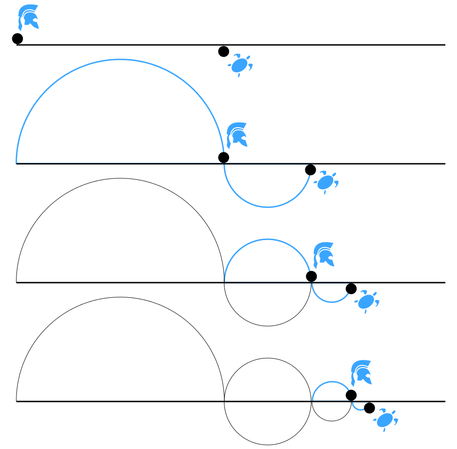
\includegraphics[scale=0.4]{img/achilles-paradox}
 \caption{阿基里斯与乌龟悖论}
 \label{fig:Achilles-paradox}
\end{figure}

但这与我们生活中的常识是不相符的。我们在小学数学课上学习过“追及问题”,通常利用相对运动加以解决。令乌龟的速度为$v_1$,阿基里斯的速度为$v_2$,则阿基里斯相对于乌龟的运动速度为$v_2 - v_1$。若乌龟在阿基里斯前方距离$s$处,则阿基里斯在$t = \frac{s}{v_2 - v_1}$时与乌龟相遇并接下来超过乌龟。但系统严密的相对运动概念要等到现代科学之父伽利略在两千多年之后才提出。芝诺的推理是如此让人信服,以至于千百年来吸引了无数学者的研究。刘易斯·卡罗尔(Lewis Carrol)、侯世达(Douglas Hofstadter)甚至拿乌龟和阿基里斯作为文学作品中的主人公。

阿基里斯与乌龟悖论的解决通常需要极限的概念。但我们手里的武器——作为分数和的小数已经足够强大到解决它。为了让推理更直观,假设阿基里斯的速度是乌龟的10倍,即$v_2 : v_1 = 10$,乌龟在阿基里斯前$s = 100$米\footnote{古希腊类似的长度单位叫做Pous,翻译为“尺”,也叫做“脚长”,是一种基于人体尺度的长度单位,大约合0.308米。}处。按照芝诺的推理,阿基里斯需要先跑完$s = 100$米,此时乌龟向前爬了$\frac{1}{10}s = 10$米;接下来阿基里斯要继续跑这10米,但乌龟又向前爬了$\frac{1}{100}s = 1$米……所以阿基里斯要跑的距离是:

\[
s(1 + \frac{1}{10} + \frac{1}{100} + \cdots) = 100\times(1 + 0.1 + 0.01 + \cdots) = 100 \times 1.11\cdots = 111.11\cdots
\]

假设阿基里斯是个“百米飞人”,只用9秒就可以跑完100米。但接下来他需要再用0.9秒跑完10米,然后再用0.09秒跑完1米……总共需要的时间是:

\begin{align*}
9 + 0.9 + 0.09 + \cdots &= 9.99\cdots = 10 \times 0.99\cdots & \\
                        &= 10 \times 1 & \text{据引理\ref{th:cycle-of-9}} \\
                        &= 10
\end{align*}

这样即使按照芝诺的推理,阿基里斯在10秒时就可以追上并超越乌龟。

\subsection{无限循环小数}
\index{无限循环小数}
为了把即约分数$\frac{b}{a}$转化为小数,我们用$b$除以$a$。有的能除尽,如$\frac{1}{2} = 0.5$、$\frac{1}{8} = 0.125$、$\frac{1}{25} = 0.4$,有的除不尽产生循环,如$\frac{1}{3} = 0.\dot{3} = 0.333\cdots$、$\frac{1}{7} = 0.\dot{1}\dot{4}\dot{2}\dot{8}\dot{5}\dot{7}$。什么时候能除尽?什么时候除不尽?这好像是一个运气问题。实际上我们的运气非常“差”,通常是除不尽的。下面的定理揭示了我们要有多幸运才能除尽。

\index{有限小数}
\begin{theorem} \label{thm:finite-decimal}
  当且仅当分数$\dfrac{b}{a} = \dfrac{b}{2^{\alpha}5^{\beta}}$时能化成有限小数,其中$\alpha$、$\beta$是非负整数。
\end{theorem}

\begin{proof}
令$n = \max(\alpha, \beta)$,即$\alpha$、$\beta$中的较大者。故$n - \alpha \geq 0$,$n - \beta \geq 0$。

\[
10^n \frac{b}{a} = \frac{2^n 5^n b}{2^{\alpha} 5^{\beta}} = 2^{n - \alpha} 5 ^{n - \beta} b
\]

一定是整数。所以$\frac{b}{a}$的小数部分有$n$位,即$0.a_1 a_2 \cdots a_n$是有限小数。

反过来,$n$位有限小数$0.a_1 a_2 \cdots a_n$展开成分数和为:

\begin{align*}
\frac{a_1}{10} + \frac{a_2}{10^2} + \cdots + \frac{a_n}{10^n} &= \frac{a_1 10^{n-1} + a_2 10^{n-2} + \cdots + a_n}{10^n} & \text{通分} \\
  &= \frac{B}{10^n} & \text{记分子为}B \\
  &= \frac{B}{2^n 5^n} = \frac{b}{a} & \text{约分}
\end{align*}

因为分母$10^n = 2^n 5^n$只有因子2和5的幂\footnote{幂在《说文解字》中来自象形文字“$\cap$”,本意是盖东西用的巾。数学中取反复覆盖的意思表达自乘。},所以约分后$a$也只有2和5的幂。
\end{proof}

有了这个结论,当我们看到一个分数的分母含有2和5以外的其它因子时,比如3、7、11……则它一定不能化成有限小数。这个定理的证明还可以扩展到$b$进制小数。如果分母含有任何不能整除$b$的因子,则除不尽,不能转换成$b$进制有限小数。所以$\frac{5}{12} = 0.41666\cdots$尽管不能化成10进制有限小数,但可以化成古巴比伦60进制小数0, 25。而$\frac{5}{14}$却不能化成60进制有限小数。特别地,形如$\frac{b}{2^n}$以外的任何即约分数都不能化成二进制有限小数,这就造成了电子计算机内部的小数计算的误差。

除此之外的分数就只能化成无限循环小数了(下一章我们将看到即约分数不可能产生无限\underdot{不}循环小数)。但我们发现有的有一位循环节,如$\frac{1}{3} = 0.\dot{3}$,有的有两位,如$\frac{5}{11} = 0.\dot{4}\dot{5}$,有的更长,如$\frac{1}{7} = 0.\dot{1}\dot{4}\dot{2}\dot{8}\dot{5}\dot{7}$,有的一开始不循环,后面才开始循环,如$\frac{5}{12} = 0.41\dot{6}$,这里面有什么规律么?

\begin{proposition}
$\dfrac{a}{9}$的小数形式是$0.\dot{a} = 0.aaa\cdots$
\end{proposition}

\begin{proof}
  \begin{align*}
    \text{令}x &= 0.\dot{a} = 0.aaa\cdots && \\
           10x &= a.aaa\cdots && \\
       10x - x &= a.aaa\cdots - 0.aaa = a && \\
            9x &= a && \\
             x &= \frac{a}{9} && \qedhere
  \end{align*}
\end{proof}

所以$\frac{1}{3} = \frac{3}{9} = 0.\dot{3} = 0.333\cdots$进一步:

\begin{proposition} \label{th:cyclic-decimal}
无限循环小数$0.\dot{a_1} \dot{a_2} \cdots \dot{a_n}$的分数形式是$\dfrac{a_1 a_2 \cdots a_n}{99 \cdots 9} = \dfrac{a_1 a_2 \cdots a_n}{10^{n+1} - 1}$。
\end{proposition}

我们把此命题的证明留作\cref{qn:cyclic-decimal}。可以用$\frac{1}{7}$验证一下:

\begin{center}
\opmul[displayshiftintermediary=all,
       voperator=bottom,
       voperation=top]{142857}{7}
\end{center}

故:
\[
0.\dot{1}\dot{4}\dot{2}\dot{8}\dot{5}\dot{7} = \frac{142857}{999999} = \frac{142857}{142857 \times 7} = \frac{1}{7}
\]

\index{循环节}
这个命题使得我们可以轻松看出$\frac{2}{11}$、$\frac{4}{33}$等分数的循环小数表示,例如$\frac{2}{11} = \frac{2 \times 9}{11 \times 9} = \frac{18}{99} = 0.\dot{1}\dot{8}$。通过这个命题还可以发现循环节长度的规律。如果$\frac{a_1 a_2 \cdots a_n}{99 \cdots 9}$约分后是$\frac{b}{a}$,那么$ak = 999 \cdots 9$。也就是说$ak + 1 = 100 \cdots 0$。因此如果$100\cdots 0$($n$个0)除以$a$的余数是1,那么$\frac{b}{a}$的循环节的长度\underdot{最长}为$n$。循环节的长度仅和分母有关\footnote{数论中的费马小定理断言,素数$p$除$10^{p-1}$的余数等于1。例如1000000除以7余1,$\frac{b}{7}$的循环节长6。尽管$10^{11-1} = 10000000000$除以11余1,但$\frac{2}{11} = 0.\dot{1}\dot{8}$的循环节长2。我们需要更多的数论知识,例如欧拉定理,才能唯一确定循环节的长度。这超出了本书的范围。参见《哈代数论》IX}。我们还需要最后一个定理来回答什么时候开始循环的问题。

\begin{theorem}\label{thm:cyclic-decimal}
即约真分数$\dfrac{b}{2^{\alpha} 5^{\beta} q}$,其中$q$不含任何2、5为因子。令$n = \max(\alpha, \beta)$,则其小数形式从$n$位后开始循环,循环节的长度是$m$,并且$10^{m+1}$除以$q$余1。
\end{theorem}

\begin{proof}
我们组合之前的证明过程。首先证明前$n$位不循环:

\[
10^n \frac{b}{2^{\alpha} 5^{\beta} q} = \frac{2^n 5^n b}{2^{\alpha} 5^{\beta} q} = \frac{2^{n - \alpha} 5^{n - \beta} b}{q} = X + \frac{b'}{q}
\]
这相当于扩大$10^n$后化带分数,其中$X$是整数部分,$0 \leq X < 10^n$。接下来由于$10^{m+1}$除以$q$余1,所以它减1后能被$q$整除:

\begin{align*}
  (10^{m+1} - 1) \frac{b'}{q} &= k b' = a_1 a_2 \cdots a_m & \text{是整数}\\
                \frac{b'}{q} &= \frac{a_1 a_2 \cdots a_m}{99\cdots9} & m\text{个}9
\end{align*}
由命题\ref{th:cyclic-decimal}知它是无限循环小数。
\end{proof}

例如$\frac{5}{12} = 0.41\dot{6}$,其中$12 = 2^2 \times 5^0 \times 3$,指数2和0的最大值是2,所以2位后开始循环;$q = 3$,循环节长1。

\begin{mdframed}

%% \begin{center}
%%  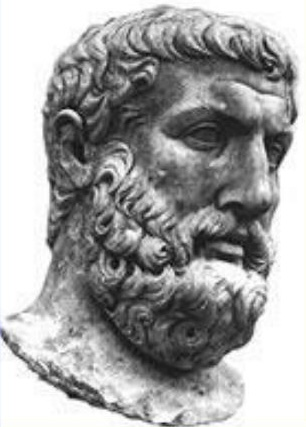
\includegraphics[scale=0.3]{img/zeno}
%%  \captionof{figure}{芝诺,约490BC - 425BC}
%%  \label{fig:Zeno-of-Elea}
%% \end{center}

\index{埃利亚的芝诺}
芝诺(约公元前490年——公元前425年),古希腊哲学家,生于意大利半岛南部的埃利亚。所以我们常称其为埃利亚的芝诺。关于他的生平,缺少可靠的文字记载。据传,他早年是一个自学成才的乡村孩子,一生经历坎坷,最终遭到一位暴君的陷害而被拘捕、拷打、直至被处死\cite{HanXueTao16}。芝诺是著名的哲学学派——埃利亚学派的代表人物之一,这一学派的领袖是芝诺的老师巴门尼德。巴门尼德认为整个世界是个不变的整体,即“不变的一”,运动、变化与多样性都只是幻象。芝诺以其悖论闻名。他一生曾巧妙地构想出40多个悖论,在流传下来的悖论中以关于运动的四个“无限微妙、无限深邃”的悖论最为著名。他提出这些悖论很可能是为他老师的哲学观点辩护。

\begin{center}
 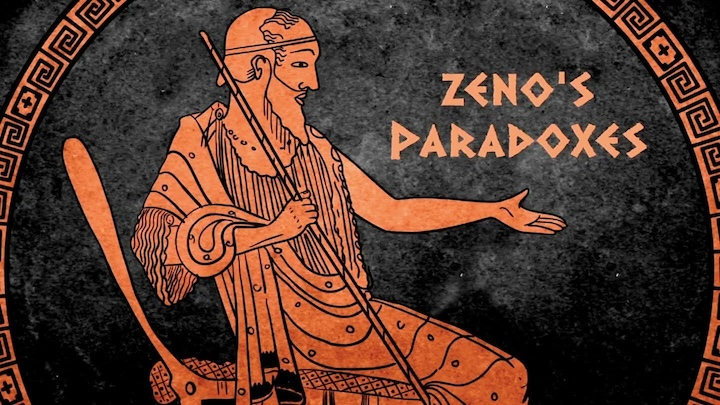
\includegraphics[scale=0.3]{img/zeno-paradox}
 \label{fig:Zeno-paradox}
\end{center}

\index{芝诺悖论!二分悖论}
除了阿基里斯与乌龟悖论外,另外三个悖论分别叫做“二分悖论”、“飞矢不动悖论”、“运动场悖论”。二分悖论的主人公是希腊神话中善于疾走的女猎手阿塔兰塔。如果阿塔兰塔想从$A$到$B$,那么她必须先走到$1/2$的位置。同样在此之前,她必须要到达$1/4$的位置。而为了到达这一位置,她必须先到达$1/8$的位置……以此类推。由于这样的中点有无限多个,阿塔兰塔永远也也无法到达目的。芝诺利用这个悖论来说明了运动根本无法发生。\cref{qn:dichotomy-paradox}要求读者扩展引理\ref{th:cycle-of-9}来解决二分和的问题。

\begin{center}
 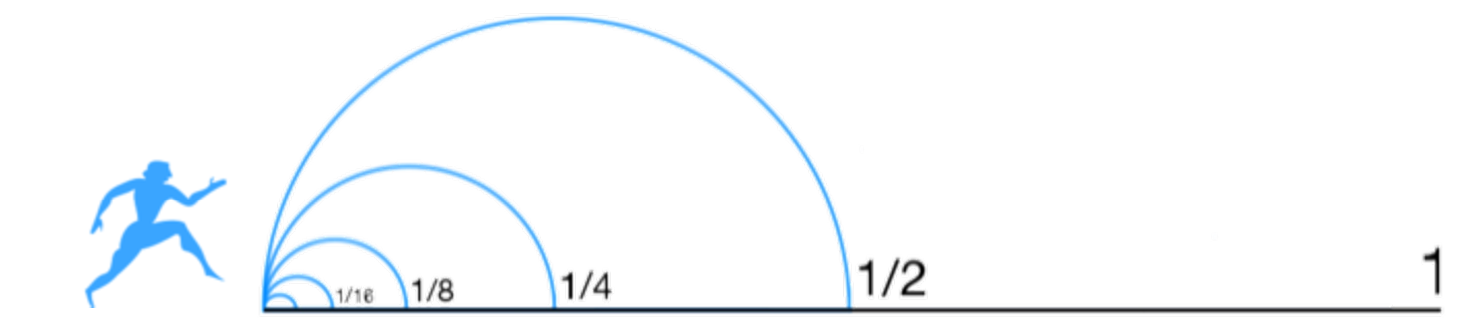
\includegraphics[scale=0.4]{img/dichotomy-paradox}
 \captionof{figure}{二分悖论}
 \label{fig:dichotomy-paradox}
\end{center}

\index{芝诺悖论!飞矢不动悖论}
飞矢不动悖论从另一个角度描述无穷导致运动无法发生。芝诺指出,任何物体停在相同的位置都不叫运动,可是飞行的箭矢在任一时刻不也是停在一个地方么?这样说来,自然飞失也是不动的。如果说前两个悖论是由于分割空间导致的,则这个悖论是由对时间的分割导致的。

\begin{center}
 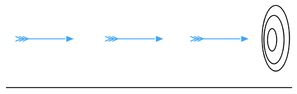
\includegraphics[scale=0.4]{img/arrow-paradox}
 \captionof{figure}{飞失不动悖论}
 \label{fig:Arrow-paradox}
\end{center}

\index{芝诺悖论!运动场悖论}
第四个悖论叫作“运动场悖论”。这一悖论主要针对时间原子论的观点,即认为存在最小的不可分割的时间单位。如\cref{fig:Moving-rows-paradox}所示,运动场中有3列人。最初他们都首尾对齐。在最小的时间单元内,A列不动,B向右移一个单位,而$\Gamma$向左移动一个单位。容易得知,相对B而言,$\Gamma$其实移动了两个单位。这就意味着,应该存在这一让$\Gamma$相对于B移动一个单位的时间。而这一时间应该是最小单位时间的一半。但如果存在不可分割的“时间原子”,那么这两个时间就是相同的,即最小时间和它的一半相等。

\begin{center}
 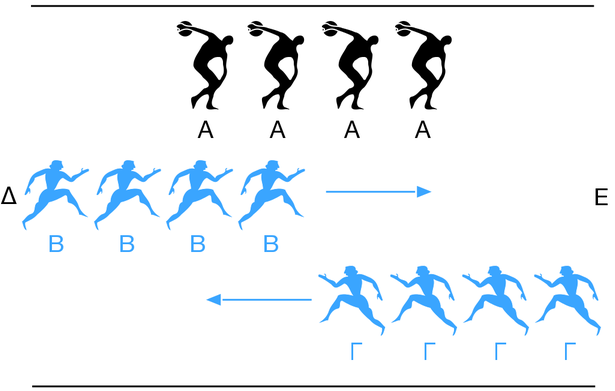
\includegraphics[scale=0.3]{img/moving-rows-paradox}
 \captionof{figure}{运动场悖论}
 \label{fig:Moving-rows-paradox}
\end{center}

芝诺悖论并不复杂,稍加琢磨就能理解。但是导出的结果却出人意料。根据生活中的常识,运动和时间是如此真实,阿基里斯不可能赶不上乌龟。可是驳倒这些悖论却并不容易,从亚里士多德到罗素,从阿基米德到赫尔曼$\cdot$外尔,都对芝诺悖论提出了各种不同的解法\cite{Britannica-Zeno-24}。芝诺悖论在当时曾给古希腊人造成深深的困惑。而芝诺悖论所涉及的对时间、空间、无限、连续、运动的看法,也都在极长的历史岁月中困扰着后来的哲学家和数学家。
\end{mdframed}

\section{数系的扩展}
在某种意义上,分数是人类在历史上第一次正式扩展我们的数系。分数看起来和0、1、2、3……大相径庭。它有两个部分:分子和分母;它抽象了多种不同的东西:小数、百分数、除法、比例$a:b$,它们本质上都是分数。尤其是后两种,它们展示出0、1、2、3……不具备的一个特性:$\frac{1}{2} = \frac{2}{4} = \frac{50}{100} = 3 \div 6 = 7:14 = \cdots$这说明一个值的分数表示是\underdot{不唯一}的。这反映了不同的除法式子可以得出相等的值(或比例)。如果要把分数加入“数”的大家庭,我们就必须解决一系列问题:

\begin{enumerate}[问题1.]
\item 哪些分数(比例)是等价的?
\item 怎样比较分数间的大小?怎样比较分数与其它数的大小?分数在数轴上的位置是什么?
\item 分数间的四则运算是怎样的?分数与其它数的四则运算是怎样的?
\item 五大运算定律对分数适用么?加法、乘法的单位元对分数的意义一样么?
\end{enumerate}

\index{等价关系} \label{sec:frac-equiv}
先看问题1,若$\frac{b}{a} = \frac{d}{c}$,两边乘以$ac$有$bc = ad$,这个结果被形象地称为“交叉相乘”(见\cref{fig:cross-mul})。在小学数学课中,我们知道比例相等时$b : a = d : c$有外项积等于内项积,即$bc = ad$,这和分数等价是一致的。在数学上,一个关系$\sim$要成为\underdot{等价关系}需要满足三个条件:

\begin{enumerate}[条件1.]
\item 自反性,即$a \sim a$。
\item 对称性,若$a \sim b$则$b \sim a$。
\item 传递性,若$a \sim b, b \sim c$则$a \sim c$。
\end{enumerate}

\index{等价关系!分数}
我们不难验证$bc = ad$是一个等价关系。首先验证自反性,比较$\frac{b}{a}$和$\frac{b}{a}$自己,显然$ab = ab$,满足自反性。其次验证对称性,如果$\frac{b}{a}$和$\frac{d}{c}$满足$bc = ad$,显然也有$ad = bc$,这样$\frac{d}{c}$和$\frac{b}{a}$之间也成立,满足对称性。最后验证传递性,若$\frac{b}{a}$和$\frac{d}{c}$满足$bc = ad$,并且$\frac{d}{c}$和$\frac{f}{e}$满足$de = cf$。等量相乘有$bcde = adcf$。因为$c \ne 0$是分母,可以消去得$bde = adf$。若$d \ne 0$也可以消去,进一步有$be = af$;否则$d = 0$,则$bc = ad = 0 = de = cf$,因此$b = f = 0$,同样有$be = af$。满足传递性。

\begin{figure}[htbp]
 \centering
 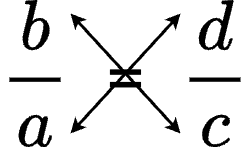
\includegraphics[scale=0.4]{img/cross-mul}
 \caption{交叉相乘}
 \label{fig:cross-mul}
\end{figure}

\index{即约分数}
有了这个等价关系,就可以判断任何两个分数(或比例)是否等价。我们可以在众多的分数表示中选取$\frac{b}{a}$,且$a, b$没有除1以外的公因子(也称为互素,记作$(a, b) = 1$)的作为\underdot{代表},称为“即约分数”。唯一的例外是0,我们选取0作为$\frac{0}{a}$的代表。这样的代表只有一个,因为若$\frac{b}{a} = \frac{d}{c}$,且各自的分子分母互素,由等价关系$bc = ad$,所以$a$整除$bc$。又因为$a$和$b$互素,所以$a$必然整除$c$;反过来由等价关系$bc = ad$还可以推出$c$整除$ad$。又因为$c$和$d$互素,所以$c$必然整除$a$。这样$a$和$c$互相能够整除对方,所以它们必然相等,即$a = c$。同理可证$b = d$,这就证明了即约分数的代表是唯一的。

也许有读者问,为什么要引入这么复杂的等价关系?为什么不直接约分看结果是否一样?古人一开始的确是自然地采用约分来判断相等的,如同上节《九章算术》中介绍的那样。并且在小学数学课上我们也是这样做的。但随着我们用分数这个武器挑战更大的数和更复杂的问题,就发现新的情况了。乘法远远比除法更容易。面对$\frac{8723}{22814}$和$\frac{143}{374}$这样的分数时,恐怕很少有人能一眼看出如何约分,即使借助计算器或使用欧几里得算法。但做乘法就快多了,用计算器很快就算出$8723 \times 374 = 3262402$并且$22814 \times 143 = 3262402$,所以它们相等。中学数学把分数拓展到了分式,我们发现这个等价关系依然好用。例如$\dfrac{x^5 - 1}{x^3 - 1}$和$\dfrac{1 + x + x^2 + x^3 + x^4}{1 + x + x^2}$,同学们对它们进行因式分解再约分通常会遇到困难\footnote{其中一个方法是:看出$1^n - 1 = 0$,所以$x-1$是$x^n-1$的一个因子。接下来用多项式长除法得出另一个因子。}。但多项式乘法却容易得多:

\begin{align*}
(x^3 - 1)(1 + x + x^2 + x^3 + x^4) &= \cancel{x^3} + \cancel{x^4} + x^5 + x^6 + x^7 - 1 - x - x^2 - \cancel{x^3} - \cancel{x^4} \\
  &= x^7 + x^6 + x^5 - x^2 - x - 1 \\
(x^5 - 1)(1 + x + x^2) &= x^5 + x^6 + x^7 - 1 - x - x^2 \\
  &= x^7 + x^6 + x^5 - x^2 - x - 1
\end{align*}

所以这两个分式是相等的。这就是数学家们为何要抽象出等价关系的概念,并精挑细选地用“交叉相乘”来判断分数、比例、分式相等。

\vspace{3mm}
对于问题2,我们可以利用《九章算术》中的办法,通过$\frac{b}{a} - \frac{d}{c}$与0的关系来判断大小。这个过程相当于通分后比较新的分子间大小。我们可以把任何整数$n$转化为$\frac{n}{1}$,这样所有的大小关系就转化为分数之间的比较。这也意味着任何一个分数都对应到数轴上的一点。对于任何多个数,包括整数、分数、小数都可以对应到数轴上的各自位置。然后从左到右整理出它们的序关系。

\vspace{3mm}
对于问题3,《九章算术》给出了分数间的四则运算规则。概括为加减先通分,再加减分子,最后约分;乘法把分子分母各自相乘、约分。一个数$n \ne 0$的倒数是$\frac{1}{n}$,因为$n\frac{1}{n} = \frac{n}{n} = 1$。如果$n$是分数$\frac{b}{a}$,它的倒数是$\frac{a}{b}$,因为$\frac{b}{a}\frac{a}{b} = 1$。分数本质上相当于除法,我们可以通过倒数在分数——除法——乘法间转换:

\[
\frac{b}{a} = b \div a = b \times 1 \div a = b \times \frac{1}{a}
\]

以及:

\[
\frac{b}{a} \div \frac{d}{c} = \frac{b}{a} \times 1 \div \frac{d}{c} = \frac{b}{a} \times \frac{c}{d}
\]

或:

\begin{align*}
\frac{b}{a} \div \frac{d}{c} = \dfrac{\quad\dfrac{b}{a}\quad}{\dfrac{d}{c}} &= \frac{bc}{ad} & \text{上下同} \times ac
\end{align*}

同样,任何整数$n$可以转化为$\frac{n}{1}$,从而将整数与分数的四则运算转化为分数间的四则运算。

\vspace{3mm}
\index{封闭运算}
对于问题4,我们发现将分数引入数系后,任何数都可表示为分数:整数$n$包括0,表示为$\frac{n}{1}$;分数、有限小数、无限循环小数表示为$\frac{b}{a}, a \ne 0$。这个数系称做\underdot{有理数},记作$\mathbb{Q}$。我们将在第4章解释这个名字的含义。在整数$\mathbb{Z}$中,每个数$x$都有相反数(加法的逆元)$-x$,但只有$\pm 1$有倒数(乘法的逆元)。在有理数$\mathbb{Q}$中,每个不等于0的数$x$都有倒数(乘法的逆元)$\frac{1}{x}$。自然数$\mathbb{N}$对加法减运算不是封闭的,例如$1 - 3 = -2 \notin \mathbb{N}$。但加减运算在整数$\mathbb{Z}$内是封闭的,任何两个整数$m, n$,总有$m \pm n \in \mathbb{Z}$。整数$\mathbb{Z}$对四则运算不是封闭的,因为$1 \div 2 = \frac{1}{2} = 0.5 \notin \mathbb{Z}$。但四则运算在有理数$\mathbb{Q}$内是封闭的,任何两个有理数$p, q$,总有$p \pm q, pq, \frac{p}{q} (q \ne 0)$都在$\mathbb{Q}$内。

可以验证五大运算定律对于分数都成立,我们这里验证加法的结合率、乘法对加法的分配律,其余三个留作\cref{qn:arithmatic-law-fraction}。
\begin{proof}
分数加法的结合律:
\begin{align*}
(\frac{b}{a} + \frac{d}{c}) + \frac{f}{e} & = \frac{bc + ad}{ac} + \frac{f}{e} = \frac{bce + ade + acf}{ace} && \\
  & = \frac{bce + (ade + acf)}{ace} & \text{对分子和用结合律} & \\
  & = \frac{b\cancel{ce}}{a\cancel{ce}} + \frac{ade + acf}{ace} && \\
  & = \frac{b}{a} + (\frac{\cancel{a}d\cancel{e}}{\cancel{a}c\cancel{e}} + \frac{\cancel{ac}f}{\cancel{ac}e}) && \\
  & = \frac{b}{a} + (\frac{d}{c} + \frac{f}{e}) && \qedhere
\end{align*}
\end{proof}

\begin{proof}
我们只证明左侧的分数分配律,右侧的证明可以利用分数乘法交换律。
\begin{align*}
  \frac{b}{a}(\frac{d}{c} + \frac{f}{e}) &= \frac{b}{a}\frac{de + cf}{ce} && \\
    &= \frac{b(de + cf)}{ace} = \frac{bde + bcf}{ace} & \text{分子用分配律} & \\
    &= \frac{bd\cancel{e}}{ac\cancel{e}} + \frac{b\cancel{c}f}{a\cancel{c}e} && \\
    &= \frac{b}{a}\frac{d}{c} + \frac{b}{a}\frac{f}{e} && \qedhere
\end{align*}
\end{proof}

\vspace{3mm}
\index{平均律}
让我们回到毕达哥拉斯追寻天籁之音的故事。发现了分数导致和谐的乐音后,如何调整里尔琴上的七根琴弦呢?如果加上第八根琴弦,那么它应该是第一根琴弦的一半,这样才能跨越八度音程。毕达哥拉斯发现纯五度音程$3:2$叠加一个纯四度音程$4:3$恰好是一个八度音程,因为:$\frac{3}{2} \times \frac{4}{3} = 2$。他用纯五度音程的比例$3:2$作为倍数,不断提高音调,得到一组等比数列:

\[
(\frac{3}{2})^{-1}, (\frac{3}{2})^0, (\frac{3}{2})^{1}, (\frac{3}{2})^2, (\frac{3}{2})^{3}, (\frac{3}{2})^4, (\frac{3}{2})^{5} = \frac{2}{3}, 1, \frac{3}{2}, \frac{9}{4}, \frac{27}{8}, \frac{81}{16}, \frac{243}{32}
\]

其中后面4个数大于2,超过了八度音程。因此毕达哥拉斯把它们每个数都除以2或4,找到其对应的前一个八度音程的数,然后重新从小到大排列得到:

\[
1, \frac{9}{8}, \frac{81}{64}, \frac{4}{3}, \frac{3}{2}, \frac{27}{16}, \frac{243}{128}, \frac{2}{1}
\]

它表示的是音阶中每个音与最低音的比例关系。为了知道每个音的相对关系,于是让相邻的两个数相除,又得到:

\[
\frac{9}{8}, \frac{9}{8}, \frac{256}{243}, \frac{9}{8}, \frac{9}{8}, \frac{9}{8}, \frac{256}{243}
\]

\index{调性}
较大的9:8叫全音,较小的256:243叫半音。这个列表就是“全、全、半、全、全、全、半”,在音乐上叫做“大调”。通常表现欢快的,阳刚的主题。而音乐上的“小调”,对应的列表移动一下是“全、半、全、全、半、全、全”。通常表现含蓄的、柔美的主题。可是有没有可能使得每个比例相同,得到完美的“平均律”呢?这超出了毕达哥拉斯所能想到的所有设计。为了达到这样的天籁之音,我们需要在一个八度音程$2:1$中设置5个全音,2个半音,共$5 \times 2 + 2 = 12$个比例,使得:

\[
1 = \alpha^0, \alpha^1, \alpha^2, \alpha^3, \alpha^4, \alpha^5, \alpha^6, \alpha^7, \alpha^8, \alpha^9, \alpha^{10}, \alpha^{11}, \alpha^{12} = 2
\]

显然$\alpha = \sqrt[12]{2}$,但它不是一个分数!让我们沿着数的旅程继续追寻天籁之音吧。

\begin{Exercise}[label={ex:fractions}]
\Question{“调和”平均值\footnote{英文harmonic mean,意为“和谐的”平均值。}的名字来自毕达哥拉斯的音乐理论。毕达哥拉斯尝试在长度为$a$和$b$的琴弦之间插入一根琴弦$h$,使得它们发出和谐的声音。他发现弦长$h$的倒数恰好在$a$和$b$的倒数正中间,即:\index{调和平均值}
\[
\frac{1}{h} - \frac{1}{a} = \frac{1}{b} - \frac{1}{h}
\]
调和平均值因此也称做倒数平均值。请根据调和平均值的定义验证:1) 在两地之间往返的平均速度是前往的速度和返回速度的调和平均值。例如从船只从南京顺流而下到达上海的平均速度是$v_1$,从上海逆流而上的平均速度是$v_2$,则往返的平均速度$v$是$v_1$与$v_2$的调和平均值。2) 在电路中并联的两个不同电阻$R_1$和$R_2$若等效于并联了\underdot{两个相同}的电阻$R$,则$R$的大小是$R_1$与$R_2$的调和平均值。(注意:$R$相当于并联电阻的2倍)
}

\Question{$\bigstar$若$p$为大于2的素数,证明$\frac{2}{p}$可\underdot{唯一}分解为两个埃及分数$\frac{2}{p} = \frac{1}{a} + \frac{1}{b} (a \ne b)$。提示:这个式子等价于$(2a - p)(2b - p) = p^2$。\label{qn:unique-decompose-r}}

\Question{证明埃尔德什——斯特劳斯猜想对所有偶数$n$成立。}

\Question{实际上我们只要证明埃尔德什——斯特劳斯猜想对于所有素数成立即可。这是为什么?}

\Question{证明埃尔德什——斯特劳斯猜想对所有$4k+3$型的素数成立。提示:利用\cref{qn:unique-decompose-r}的结论。}

\Question{$\bigstar$找出三个儿子按照$\frac{1}{a}$、$\frac{1}{b}$、$\frac{1}{c}$分配$n$个动物的所有可能数值和比例。要求大儿子分得的财产多于二儿子,二儿子分得的财产多于小儿子。恰好借来一只动物后可以分好并余下一只动物。如果你会编程,可以用计算机枚举出所有解。但此题要求手工找出所有可能的$n, a, b, c$。提示:本题本质是求方程$\frac{n}{n+1} = \frac{1}{a} + \frac{1}{b} + \frac{1}{c}, a < b < c$的所有正整数解。三儿子至少分得一只动物,那么$n$的最小值是多少?你能据此推出$a$不可能超过3,因而只能是2么?\label{qn:three-sons}}

\Question{$\bigstar$由于$0.999\cdots = 1$,所以任何有限小数有两种表示:$X.a_1a_2 \cdots a_m000\cdots$和$X.a_1a_2 \cdots b999\cdots$,其中$b = a_m - 1$,$X$是整数部分。证明除了这种情况外,任何数值$x$的小数表示是唯一的,其中$0 < x < 1$。}

\Question{证明无限循环小数$0.\dot{a_1} \dot{a_2} \cdots \dot{a_n}$的分数形式是$\frac{a_1 a_2 \cdots a_n}{99 \cdots 9} = \frac{a_1 a_2 \cdots a_n}{10^{n+1} - 1}$。\label{qn:cyclic-decimal}}

\Question{利用分数和引理\ref{th:cycle-of-9}解释:如果阿塔兰塔先跑完全程的$\frac{1}{2}$,接下来再跑完剩余的一半,即$\frac{1}{4}$,然后不断跑完剩余路程的一半,则她最终可以跑完全程。提示:考虑二进制分数和。\label{qn:dichotomy-paradox}}

\Question{验证分数的加法交换律、乘法交换律,乘法结合率。\label{qn:arithmatic-law-fraction}}
\end{Exercise}

\begin{Answer}[ref={ex:fractions}]
\Question{根据调和平均值的原始定义:

\begin{align*}
\frac{1}{h} - \frac{1}{a} &= \frac{1}{b} - \frac{1}{h}    \\
\frac{2}{h} &= \frac{1}{a} + \frac{1}{b} \\
 h &= \frac{2}{\frac{1}{a} + \frac{1}{b}} = \frac{2ab}{a + b}
\end{align*}

令两地间距离为$s$,往返的时间分别为:往$t_1 = \frac{s}{v_1}$、返$t_2 = \frac{s}{v_2}$。平均速度为:
\begin{align*}
  v & = \frac{2s}{t_1 + t_2} = \frac{2\cancel{s}}{\frac{\cancel{s}}{v_1} + \frac{\cancel{s}}{v_2}}
    = \frac{2}{\frac{1}{v_1} + \frac{1}{v_2}} = \frac{2v_1 v_2}{v_1 + v_2}
\end{align*}

恰好是$v_1$和$v_2$的调和平均值。另外,根据往返总时间等于去的时间加返回时间:$\frac{2s}{v} = \frac{s}{v_1} + \frac{s}{v_2}$,两边约去路程$s$就得到$\frac{2}{v} = \frac{1}{v_1} + \frac{1}{v_2}$。恰好也是上边调和平均值$\frac{2}{h} = \frac{1}{a} + \frac{1}{b}$的形式。

\begin{center}
 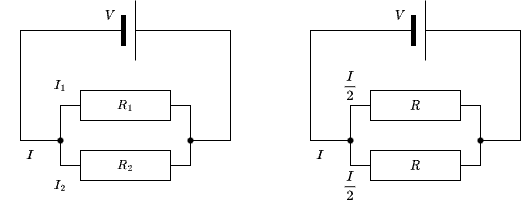
\includegraphics[scale=0.4]{img/harmonic-meanr}
 \captionof{figure}{电阻并联}
 \label{fig:harmonic-meanr}
\end{center}

如\cref{fig:harmonic-meanr}所示,左右电路等效时,加载同样的电压,流过的总电流相等,即:

\begin{align*}
\frac{I}{2} + \frac{I}{2} &= I_1 + I_2 \\
2\frac{\cancel{V}}{R} &= \frac{\cancel{V}}{R_1} + \frac{\cancel{V}}{R_2} \\
\frac{2}{R} &= \frac{1}{R_1} + \frac{1}{R_2} \\
R &= \frac{2}{\frac{1}{R_1} + \frac{1}{R_2}} = \frac{2R_1 R_2}{R_1 + R_2}
\end{align*}
所以图中右侧每个电阻等于$R_1$和$R_2$的调和平均值。
}

\Question{若$p$为大于2的素数,证明$\frac{2}{p}$可唯一分解为两个埃及分数$\frac{2}{p} = \frac{1}{a} + \frac{1}{b} (a \ne b)$。

  \begin{proof}
  上式等价于$(2a - p)(2b - p) = p^2$,我们可验证如下:
  \begin{align*}
  \frac{2}{p} & = \frac{1}{a} + \frac{1}{b} = \frac{a+b}{ab} & \text{通分} \\
  2ab & = pa + pb & p, a, b\text{是分母,不为}0 \\
  4ab - 2pa - 2pb & = 0 & \text{移项} \times 2 \\
  4ab - 2pa - 2pb + p^2 & = p^2 & \text{两边} + p^2 \\
  (2a - p)(2b - p) & = p^2 & \text{因式分解}
  \end{align*}
  因为$p$是素数,$p^2$的因子只有1、$p$、$p^2$。由$a \ne b$可以排除掉$p$,所以$2a - p = 1$,$2b - p = p^2$,即:
  \[
  a = \frac{p+1}{2}, b = \frac{p(p+1)}{2}
  \]
  因为$p$是奇素数,所以$a$是整数。因此:
  \[
  \frac{2}{p} = \frac{1}{\frac{1}{2}(p + 1)} + \frac{1}{\frac{1}{2}p(p+1)} \qedhere
  \]
  \end{proof}
}

\Question{%证明埃尔德什——斯特劳斯猜想对所有偶数$n$成立。
令$n = 2m$,则$\frac{4}{2m} = \frac{2}{m}$,这就是\cref{th:decompose-of-2-n}。
}

\Question{ %实际上我们只要证明埃尔德什——斯特劳斯猜想对于所有素数成立即可。这是为什么?
注意到:\[
\frac{4}{mp} = \frac{1}{ma} + \frac{1}{mb} + \frac{1}{mc}
\]
}
\Question{%证明埃尔德什——斯特劳斯猜想对所有$4k+3$型的素数成立。
  \begin{proof}
    利用\cref{qn:unique-decompose-r}的结论
    \begin{align*}
      \frac{2}{p} &= \frac{1}{\frac{1}{2}(p + 1)} + \frac{1}{\frac{1}{2}p(p + 1)} && \\
      \frac{4}{p} &= \frac{2}{\frac{1}{2}(p + 1)} + \frac{2}{\frac{1}{2}p(p + 1)} & \text{左右} \times 2 & \\
      \frac{4}{4k + 3} &= \frac{2}{\frac{1}{2}(4k + 4)} + \frac{2}{\frac{1}{2}(4k + 3)(4k + 4)} & \text{带入} p = 4k + 3 & \\
                       &= \frac{1}{k + 1} + \frac{1}{(4k + 3)(k + 1)} & & \\
                       &= \frac{1}{k + 2} + \frac{1}{(k + 1)(k + 2)} + \frac{1}{(4k + 3)(k + 1)} & \text{由\cref{th:egyptian-fraction-split}} & \qedhere
    \end{align*}
  \end{proof}
}

\Question{%找出三个儿子按照$\frac{1}{a}$、$\frac{1}{b}$、$\frac{1}{c}$分配$n$个动物的所有可能数值和比例。要求大儿子分得的财产多于二儿子,二儿子分得的财产多于小儿子。恰好借来一只动物后可以分好并余下一只动物。

我们先给出一个纯数学解法,然后再给出用计算机穷举的解法。读者朋友们可以加以对比。本题本质上是求方程
\[
\frac{n}{n+1} = \frac{1}{a} + \frac{1}{b} + \frac{1}{c}, a < b < c
\]
的所有正整数解。即借来一只后,把$n+1$只动物分成三份$\frac{n + 1}{a}$、$\frac{n + 1}{b}$、$\frac{n + 1}{c}$。它们的和恰好是$n$,因而可以把剩余的那一只归还。为了简洁,我们令$n' = n + 1$,表示借来一只动物后的数量,把上述方程改写为:

\be
\frac{n'-1}{n'} = \frac{1}{a} + \frac{1}{b} + \frac{1}{c}
\label{eq:equation-of-inherit}
\ee

最后只要把$n'$减一就可以了。借来一只动物后能恰好分配,意味着$a, b, c$都能整除$n'$。我们先证明一个重要的结论:大儿子只能分得$\frac{1}{2}$的财产,即$a$只能等于2。
\begin{proof}
若$a \geq 3$,由于$a < b < c$,所以:

\[
\frac{1}{a} + \frac{1}{b} + \frac{1}{c} \leq \frac{1}{3} + \frac{1}{4} + \frac{1}{5} = \frac{47}{60}
\]

小儿子至少分得1只;二儿子分得的比小儿子多,所以至少分得2只;同理,大儿子至少分得3只动物,再加上借来的一只。所以$n' > 3 + 2 + 1 = 6$。于是:

\[
\frac{n'-1}{n'} = 1 - \frac{1}{n'} > 1 - \frac{1}{6} = \frac{5}{6} = \frac{50}{60} > \frac{47}{60} \geq \frac{1}{a} + \frac{1}{b} + \frac{1}{c}
\]

也就是说$a \geq 3$时,方程\cref{eq:equation-of-inherit}不可能成立。所以$a$只能是2。
\end{proof}

问题于是就化简为,求方程
\[
\frac{n'-1}{n'} = \frac{1}{2} + \frac{1}{b} + \frac{1}{c}
\]
的正整数解。我们接下来证明$b$只能是3和4,从而进一步化简问题:

\begin{proof}
如果$b \geq 5$,由于$b < c$,故:

\[
\frac{1}{a} + \frac{1}{b} + \frac{1}{c} \leq \frac{1}{2} + \frac{1}{5} + \frac{1}{6} = \frac{13}{15} \approx 0.87
\]

由于$a, b, c$都能整除$n'$,而$a = 2$,所以$n'$必然是偶数。我们上面推出$n' > 6$,比6大的第一个偶数是8。因此:

\[
\frac{n'-1}{n'} = 1 - \frac{1}{n'} \geq 1 - \frac{1}{8} = \frac{7}{8} = 0.875 > 0.87 \geq \frac{1}{a} + \frac{1}{b} + \frac{1}{c}
\]

也就是说$b \geq 5$时,方程\cref{eq:equation-of-inherit}不可能成立。所以$b$只能是3或4。
\end{proof}

\begin{enumerate}[情况1)]
\item $a = 2, b = 3$
  \begin{align*}
    \frac{n'-1}{n'} &= \frac{1}{2} + \frac{1}{3} + \frac{1}{c} \\
    1 - \frac{1}{n'} &= \frac{5}{6} + \frac{1}{c} \\
    \frac{1}{6} &= \frac{1}{n'} + \frac{1}{c}
  \end{align*}
  由于$a = 2, b = 3$都整除$n'$,所以6整除$n'$。不妨设$n' = 6k$,其中$k$为大于1的整数(因为我们前面确定了$n'$最小是8)。代入上式,整理得:
  \[
  k = \frac{c}{c - 6} \geq 2
  \]
  解不等式$\frac{c}{c - 6} \geq 2$得$c \leq 12$。同时分母$c-6$是正数,所以$c > 6$。这样$c$的值只可能是$7, 8, 9, \cancel{10}, \cancel{11}, 12$。其中10,11不可能,因为此时$k = \frac{c}{c - 6}$不是整数。我们得到4个解:
  \begin{align*}
  a &= 2, b = 3, c = 7, n' = 42 & 42\frac{1}{2} + 42\frac{1}{3} + 42\frac{1}{7} &= 21 + 14 + 6 = 41 \\
  a &= 2, b = 3, c = 8, n' = 24 & 24\frac{1}{2} + 24\frac{1}{3} + 24\frac{1}{8} &= 12 + 8 + 3 = 23 \\
  a &= 2, b = 3, c = 9, n' = 18 & 18\frac{1}{2} + 18\frac{1}{3} + 18\frac{1}{9} &= 9 + 6 + 2 = 17 \\
  a &= 2, b = 3, c = 12, n' = 12 & 12\frac{1}{2} + 12\frac{1}{3} + 12\frac{1}{12} &= 6 + 4 + 1 = 11
  \end{align*}
\item $a = 2, b = 4$
  \begin{align*}
    \frac{n'-1}{n'} &= \frac{1}{2} + \frac{1}{4} + \frac{1}{c} \\
    1 - \frac{1}{n'} &= \frac{3}{4} + \frac{1}{c} \\
    \frac{1}{4} &= \frac{1}{n'} + \frac{1}{c}
  \end{align*}
  由于$a = 2, b = 4$都整除$n'$,所以4整除$n'$。不妨设$n' = 4k$,其中$k \geq 2 $为整数(同理$n'$最小是8)。代入上式,整理得:
  \[
  k = \frac{c}{c - 4} \geq 2
  \]
  解不等式$\frac{c}{c - 2} \geq 2$得$c \leq 8$。同时分母$c-4$是正数,所以$c > 4$。这样$c$的值只可能是$5, 6, \cancel{7}, 8$。其中7不可能,因为此时$k = \frac{c}{c - 4}$不是整数。我们得到3个解:
  \begin{align*}
  a &= 2, b = 4, c = 5, n' = 20 & 20\frac{1}{2} + 20\frac{1}{4} + 20\frac{1}{5} &= 10 + 5 + 4 = 19 \\
  a &= 2, b = 4, c = 6, n' = 12 & 12\frac{1}{2} + 12\frac{1}{4} + 12\frac{1}{6} &= 6 + 3 + 2 = 11 \\
  a &= 2, b = 4, c = 8, n' = 8 & 8\frac{1}{2} + 8\frac{1}{4} + 8\frac{1}{8} &= 4 + 2 + 1 = 7
  \end{align*}
\end{enumerate}
注意到两种情况都有分11+1只动物的可能,但分配比例不同。总共有7个解。

\vspace{3mm}
用计算机求解时,可以让机器枚举所有可能的$a, b, c$。判断其倒数和是否满足$\frac{n + 1}{n}$的形式。显然,$a$从2开始,依次尝试2、3、4……并且由于$a < b < c$,所以我们从$a+1$开始枚举$b$,从$b + 1$开始枚举$c$。接下来我们需要估计$a, b, c$的一个上限,使得枚举的过程可以结束。因为$a < b < c$,所以$c$的上限一定也是$a, b$的上限。此外,三儿子最少分到1只动物,所以$c \leq n'$。从\cref{eq:equation-of-inherit}可以推出:

\begin{align*}
  1 - \frac{1}{n'} &= \frac{1}{a} + \frac{1}{b} + \frac{1}{c} \\
  1 - \frac{1}{n'} - \frac{1}{c} &= \frac{1}{a} + \frac{1}{b} \leq \frac{1}{2} + \frac{1}{3} = \frac{5}{6} \\
  \frac{1}{6} &\leq \frac{1}{n'} + \frac{1}{c} \leq \frac{1}{c} + \frac{1}{c} & \text{三儿子至少分得一只,故} \frac{1}{n'} \leq \frac{1}{c} \\
  \frac{1}{6} &\leq \frac{2}{c} \Rightarrow c \leq 12
\end{align*}

因此枚举的上限是12。其次从$1 - \frac{1}{n'} = \frac{1}{a} + \frac{1}{b} + \frac{1}{c}$还可以解出$n' = \frac{abc}{abc - ab - bc - ac}$,如果其分母不为0,且$a, b, c$都整除$n'$,则找到了一组解。\cref{fig:inherit-program}给出了例子程序。

\begin{center}
 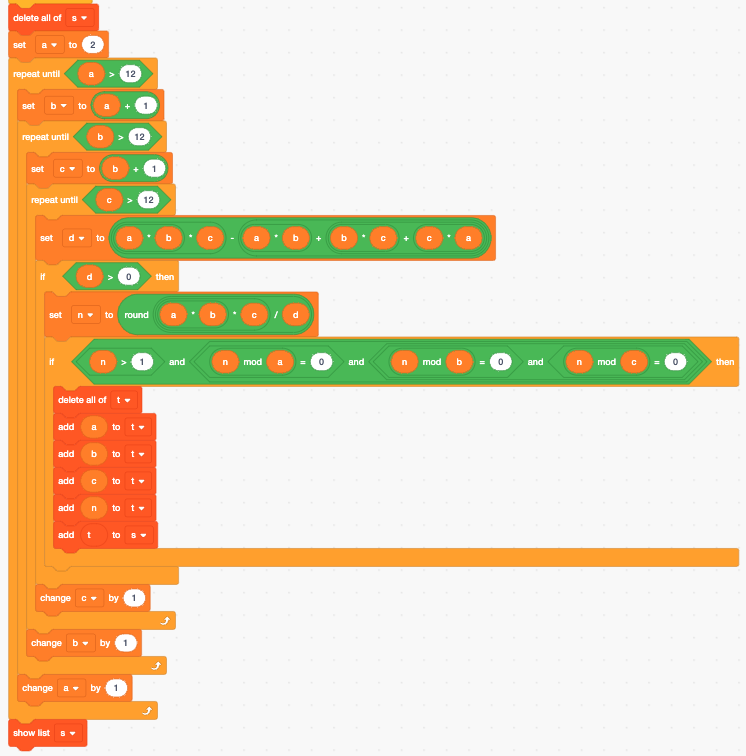
\includegraphics[scale=0.4]{img/inherit-program}
 \captionof{figure}{三子继承问题的Scratch程序}
 \label{fig:inherit-program}
\end{center}

下面是对应的Haskell例子程序。

\begin{Haskell}[frame = single]
[(a, b, c, n) | a <- [2..10], b <- [a+1..11], c <- [b+1..12],
     let d = a*b*c - a*b - b*c - a*c, d > 0,
     let n = a*b*c `div` d, n > 1,
         n `mod` a == 0, n `mod` b == 0, n `mod` c == 0]
\end{Haskell}
}

\Question{%$\bigstar$证明任何数值$x$的小数表示是唯一的,其中$0 < x < 1$。

  \begin{proof}
    用反证法,令:
\be
\frac{a_1}{10} + \frac{a_2}{100} + \cdots = \frac{b_1}{10} + \frac{b_2}{100} + \cdots
\label{eq:decimal-a-eq-b}
\ee
设$a_n$和$b_n$是第一对不相等的。$|a_n - b_n| \geq 1$。于是:
\begin{align*}
\frac{a_1}{10} + \frac{a_2}{100} + \cdots - (\frac{b_1}{10} + \frac{b_2}{100} + \cdots) & \geq \frac{1}{10^n} - (\frac{|a_{n+1} - b_{n+1}|}{10^{n+1}} + \frac{|a_{n+2} - b_{n+2}|}{10^{n+2}} + \cdots) \\
  & \geq \frac{1}{10^n} - (\frac{9}{10^{n+1}} + \frac{9}{10^{n+2}} + \cdots) \\
  & = \frac{1}{10^n} - \frac{1}{10^n}(0.99\cdots) = 0
\end{align*}

这与\cref{eq:decimal-a-eq-b}矛盾。
  \end{proof}
}

\Question{%%证明无限循环小数$0.\dot{a_1} \dot{a_2} \cdots \dot{a_n}$的分数形式是$\frac{a_1 a_2 \cdots a_n}{99 \cdots 9} = \frac{a_1 a_2 \cdots a_n}{10^{n+1} - 1}$。

  \begin{proof}
    \begin{align*}
    \text{设} x &= 0.\dot{a_1} \dot{a_2} \cdots \dot{a_n} \\
    10^n x & = a_1a_2\cdots a_n . \dot{a_1} \dot{a_2} \cdots \dot{a_n} \\
    10^n x - x &= a_1a_2\cdots a_n \\
    x &= \frac{a_1a_2\cdots a_n}{10^n - 1} = \frac{a_1a_2\cdots a_n}{99 \cdots 9} && \qedhere
    \end{align*}
  \end{proof}
}

\Question{%%利用分数和解释:如果阿塔兰塔先跑完全程的$\frac{1}{2}$,接下来再跑完剩余的一半,即$\frac{1}{4}$,然后不断跑完剩余路程的一半,则她最终可以跑完全程。

十进制无限循环小数$0.99\cdots = 1$,对应的二进制无限循环小数$0.11\cdots = 1$。证明与十进制类似:
\begin{proof}
  \begin{align*}
    x &= 0.11\cdots & 2x &= 1.11\cdots \\
    x & = 2x - x = 1 & & \qedhere
  \end{align*}
\end{proof}
阿塔兰塔先跑到$\frac{1}{2}$处,即二进制0.1处;再跑到$\frac{1}{4}$处,即二进制0.01处……她跑过的路程和等于二进制小数和:
\[
0.1 + 0.01 + 0.001 + \cdots = 0.11\cdots = 1
\]
}

\Question{%%验证分数的加法交换律、乘法交换律,乘法结合率。
加法交换律:
\begin{align*}
  \frac{b}{a} + \frac{d}{c} &= \frac{bc + ad}{ac} &\text{通分} \\
  &= \frac{ad + bc}{ac} & \text{分子用整数加法交换律} \\
  &= \frac{ad}{ac} + \frac{bc}{ac} = \frac{d}{c} + \frac{b}{a}
\end{align*}

乘法交换律:
\[
\frac{b}{a} \times \frac{d}{c} = \frac{bd}{ac} = \frac{db}{ca} = \frac{d}{c} \times \frac{b}{a}
\]

乘法结合律:
\[
\frac{b}{a} \times \frac{d}{c} \times \frac{f}{e} = \frac{bdf}{ace} = \frac{b(df)}{a(ce)} = \frac{b}{a}\frac{df}{cd} = \frac{b}{a} \times (\frac{d}{c} \times \frac{f}{e})
\]
}
\end{Answer}

\ifx\wholebook\relax \else
\section{参考答案}
\shipoutAnswer

\section{埃及分数分解算法}
\subimport{inc/}{decomposition-zh-cn}

\begin{thebibliography}{99}
\subimport{inc/}{bib-zh-cn}
\end{thebibliography}

\expandafter\enddocument
\fi
